\documentclass{article}

\usepackage{arxiv}

\usepackage[utf8]{inputenc} % allow utf-8 input
\usepackage[T1]{fontenc}    % use 8-bit T1 fonts
\usepackage{lmodern}        % https://github.com/rstudio/rticles/issues/343
\usepackage{hyperref}       % hyperlinks
\usepackage{url}            % simple URL typesetting
\usepackage{booktabs}       % professional-quality tables
\usepackage{amsfonts}       % blackboard math symbols
\usepackage{nicefrac}       % compact symbols for 1/2, etc.
\usepackage{microtype}      % microtypography
\usepackage{lipsum}
\usepackage{graphicx}

\title{Estimating Nonlinear Selection on \linebreak Behavioral Reaction
Norms}

\author{
    Jordan S. Martin
   \\
    Human Ecology Group, Institute of Evolutionary Medicine \\
    University of Zurich \\
   \\
  \texttt{\href{mailto:jordan.martin@uzh.ch}{\nolinkurl{jordan.martin@uzh.ch}}} \\
  }


% Pandoc citation processing
\newlength{\csllabelwidth}
\setlength{\csllabelwidth}{3em}
\newlength{\cslhangindent}
\setlength{\cslhangindent}{1.5em}
% for Pandoc 2.8 to 2.10.1
\newenvironment{cslreferences}%
  {}%
  {\par}
% For Pandoc 2.11+
\newenvironment{CSLReferences}[3] % #1 hanging-ident, #2 entry spacing
 {% don't indent paragraphs
  \setlength{\parindent}{0pt}
  % turn on hanging indent if param 1 is 1
  \ifodd #1 \everypar{\setlength{\hangindent}{\cslhangindent}}\ignorespaces\fi
  % set entry spacing
  \ifnum #2 > 0
  \setlength{\parskip}{#2\baselineskip}
  \fi
 }%
 {}
\usepackage{calc} % for calculating minipage widths
\newcommand{\CSLBlock}[1]{#1\hfill\break}
\newcommand{\CSLLeftMargin}[1]{\parbox[t]{\csllabelwidth}{#1}}
\newcommand{\CSLRightInline}[1]{\parbox[t]{\linewidth - \csllabelwidth}{#1}}
\newcommand{\CSLIndent}[1]{\hspace{\cslhangindent}#1}

\usepackage{amsmath, xparse, mathtools, upgreek}
\usepackage{lineno}
\linenumbers
\usepackage{hyperref}
\usepackage[labelfont=bf]{caption}
\hypersetup{ colorlinks=true, linkcolor=black, citecolor=black, filecolor=black, urlcolor=black}


\begin{document}
\maketitle

\def\tightlist{}


\begin{abstract}
Individuals' behavioral strategies are often well described by reaction
norms, which are functions predicting repeatable patterns of
personality, plasticity, and predictability across an environmental
gradient. Reaction norms can be readily estimated using mixed-effects
models and play a key role in current theories of adaptive individual
variation. Unfortunately, however, it remains challenging to assess the
effects of reaction norms on fitness-relevant outcomes, due to the high
degree of uncertainty in random effect estimates of reaction norm
parameters, also known as best linear unbiased predictors (BLUPs).
Current approaches to this problem do not provide a generalized solution
for modelling reaction norm effects with nonlinear structure, such as
stabilizing, disruptive, balancing, and/or correlational selection,
which are necessary for testing adaptive theory of individual variation.
To address this issue, I present a novel solution for straightforward
and unbiased estimation of linear and nonlinear reaction norm effects on
fitness, applicable to both Gaussian and non-Gaussian measurements. This
solution involves specifying BLUPs as random effects on behavior and
fixed effects on fitness within a Bayesian multi-response model. By
simultaneously accounting for uncertainty in reaction norm parameters
and their causal effects on other measures, the risks accompanying
classical approaches to BLUPs can be effectively avoided. I also
introduce a new method for visualizing the consequences of multivariate
selection on reaction norms. Simulations are then used to validate that
the proposed models provide unbiased estimates across realistic
parameter values, and an extensive coding tutorial is provided to aid
researchers in applying this method to their own datasets in R.
\end{abstract}

\keywords{
    mixed-effects
   \and
    multivariate
   \and
    Bayesian
   \and
    reaction norm
   \and
    adaptation
   \and
    individuality
  }

\hypertarget{introduction}{%
\section{Introduction}\label{introduction}}

A population will evolve by natural selection whenever heritable
variation occurs in fitness-relevant phenotypes
(\protect\hyperlink{ref-Darwin}{Darwin 1859}). Individual differences in
behavior are, therefore, a fundamental ingredient for adaptive
behavioral evolution. Across taxa, repeatable individual variation is
observed not only in animals' average behavior
(\protect\hyperlink{ref-Bell2009}{Bell, Hankison, and Laskowski 2009}),
but also in the degree of behavioral responsiveness they exhibit toward
the environment (\protect\hyperlink{ref-Ding2010}{Dingemanse et al.
2010}; \protect\hyperlink{ref-Stamps2016}{Stamps 2016}), as well as in
the intra-individual variability of their behavior across time
(\protect\hyperlink{ref-Biro2013}{Biro and Adriaenssens 2013};
\protect\hyperlink{ref-Westneat2015}{Westneat, Wright, and Dingemanse
2015}). These respective patterns of personality, plasticity, and
predictability represent distinct but often integrated components of the
behavioral reaction norms (RNs) within a population (see \textbf{Figure
\ref{fig:fig1}}), which are functions expressing individual-specific
behavioral strategies across an environmental gradient
(\protect\hyperlink{ref-Ding2010}{Dingemanse et al. 2010};
\protect\hyperlink{ref-McNamara2020}{McNamara and Leimar 2020}). The
evolution of such function-valued traits is currently a central area of
research within evolutionary ecology
(\protect\hyperlink{ref-Gomulk2018}{Gomulkiewicz et al. 2018}), which
has led to a host of methodological innovations for estimating the RNs
of complex traits subject to measurement error
(\protect\hyperlink{ref-DingDocht2013}{Dingemanse and Dochtermann 2013};
\protect\hyperlink{ref-Martin2021}{Martin and Jaeggi 2021}), as well as
the development of a rich theoretical framework for explaining the
adaptive processes maintaining individual variation in RNs within
populations (\protect\hyperlink{ref-Dall2014}{Dall and Griffith 2014};
\protect\hyperlink{ref-Sih2015}{Sih et al. 2015};
\protect\hyperlink{ref-Wolf2010}{Wolf and Weissing 2010}). Attention to
RNs has also increased in related fields of inquiry such as personality
psychology (\protect\hyperlink{ref-Nettle2010}{Nettle and Penke 2010})
and evolutionary anthropology (\protect\hyperlink{ref-Jaeggi2016}{Jaeggi
et al. 2016}), suggesting that an integrative framework for studying the
evolution of RNs will benefit research on individuality more generally.

For labile phenotypes such as behavior, hormones, and cognition, the
magnitude of repeatable between-individual variation in measurements is
generally modest in comparison to the total phenotypic variation
observed across space and time (\protect\hyperlink{ref-Bell2009}{Bell,
Hankison, and Laskowski 2009};
\protect\hyperlink{ref-Cauch2018}{Cauchoix et al. 2018};
\protect\hyperlink{ref-Fanson2019}{Fanson and Biro 2015}). This is
unsurprising, given that these traits are often the primary mechanisms
by which organisms can flexibly respond to ephemeral and stochastic
variation in their local environments, such as by up-regulating
circulating testosterone in response to social challenges
(\protect\hyperlink{ref-Eis2011}{Eisenegger, Haushofer, and Fehr 2011}),
or by temporarily inducing a fear state in response to odor cues of
predation (\protect\hyperlink{ref-Mathuru2012}{Mathuru et al. 2012}). As
such, single measurements of these phenotypes are poor indicators of the
underlying between-individual differences that are targeted by
selection, and tend to instead reflect various sources of
within-individual environmental heterogeneity
(\protect\hyperlink{ref-Brommer2013}{Brommer 2013};
\protect\hyperlink{ref-DingDocht2013}{Dingemanse and Dochtermann 2013}).
Despite the unfortunate fact that many empirical studies still confound
these distinct sources of trait (co)variation
(\protect\hyperlink{ref-Niem2018}{Niemelä and Dingemase 2018};
\protect\hyperlink{ref-Roy2018}{Royauté et al. 2018}), the necessity of
longitudinal data for studying RNs is increasingly appreciated and
enforced within behavioral ecology
(\protect\hyperlink{ref-Ding2020}{Dingemanse and Wright 2020}). With the
appropriate application of generalized mixed-effect models (GLMMs), such
repeated measures data can then be used to estimate the unobserved but
statistically identifiable RNs underlying raw trait measurements, thus
effectively partitioning stochastic effects and measurement error from
repeatable sources of between-individual variation
(\protect\hyperlink{ref-DingDocht2013}{Dingemanse and Dochtermann 2013};
\protect\hyperlink{ref-Martin2021}{Martin and Jaeggi 2021};
\protect\hyperlink{ref-Naka2010}{Nakagawa and Schielzeth 2010};
\protect\hyperlink{ref-Nus2007}{Nussey, Wilson, and Brommer 2007}).

GLMMs are a powerful tool not only for estimating RNs from empirical
data using random effects, but also for subsequently modeling the fixed
effects of personality, plasticity, and predictability on fitness and
other biological outcomes of interest. Nevertheless, although GLMMs
provide a quite robust modeling framework
(\protect\hyperlink{ref-Schiel2020}{Schielzeth et al. 2020}), they can
only give as much information about RNs and their effects as the model
assumptions and empirical data provided to them. For labile phenotypes
like behavior, this means that the predicted random effect values of RN
parameters, also known as best linear unbiased predictors (BLUPs), are
often inferred with non-trivial degrees of statistical uncertainty. The
use of BLUP point estimates to predict outcomes in another response
model will, therefore, artificially reduce uncertainty in the estimated
effects of RNs and increase the risk of false positives (see
\protect\hyperlink{ref-Hadfield2010}{Hadfield et al. 2010} for a
detailed treatment). Previous solutions to this problem have provided
effective antidotes to the anti-conservative inference encouraged by
ignoring uncertainty in BLUPs (\protect\hyperlink{ref-Hous2017}{Houslay
and Wilson 2017}). However, these solutions also reduce empiricists'
capacity to effectively model the nonlinear effects of RNs on
fitness-relevant outcomes, which is necessary for understanding the
degree to which natural selection is actively maintaining or diminishing
individual variation in behavior. The present study therefore introduces
a new method to facilitate unbiased estimation of nonlinear RN effects
within a Bayesian GLMM framework. The proposed solution is first
motivated through a brief discussion of current approaches to the misuse
of BLUPs and their benefits and limitations. I then formally introduce
the proposed method along with a novel approach to visualizing the
effects of multivariate selection on reaction norms. I also provide R
code (\protect\hyperlink{ref-Rbase}{R Core Team 2020}) and tutorials on
the accompanying Github repository for this manuscript
\href{https://github.com/Jordan-Scott-Martin/Selection-on-RNs}{(https://github.com/Jordan-Scott-Martin/Selection-on-RNs)},
demonstrating how to estimate these models with the Stan statistical
programming language (\protect\hyperlink{ref-Stan}{Carpenter et al.
2017}). These tutorials will aid researchers in investigating nonlinear
RN effects with their own datasets.

\begin{figure}
\hspace*{-1cm}
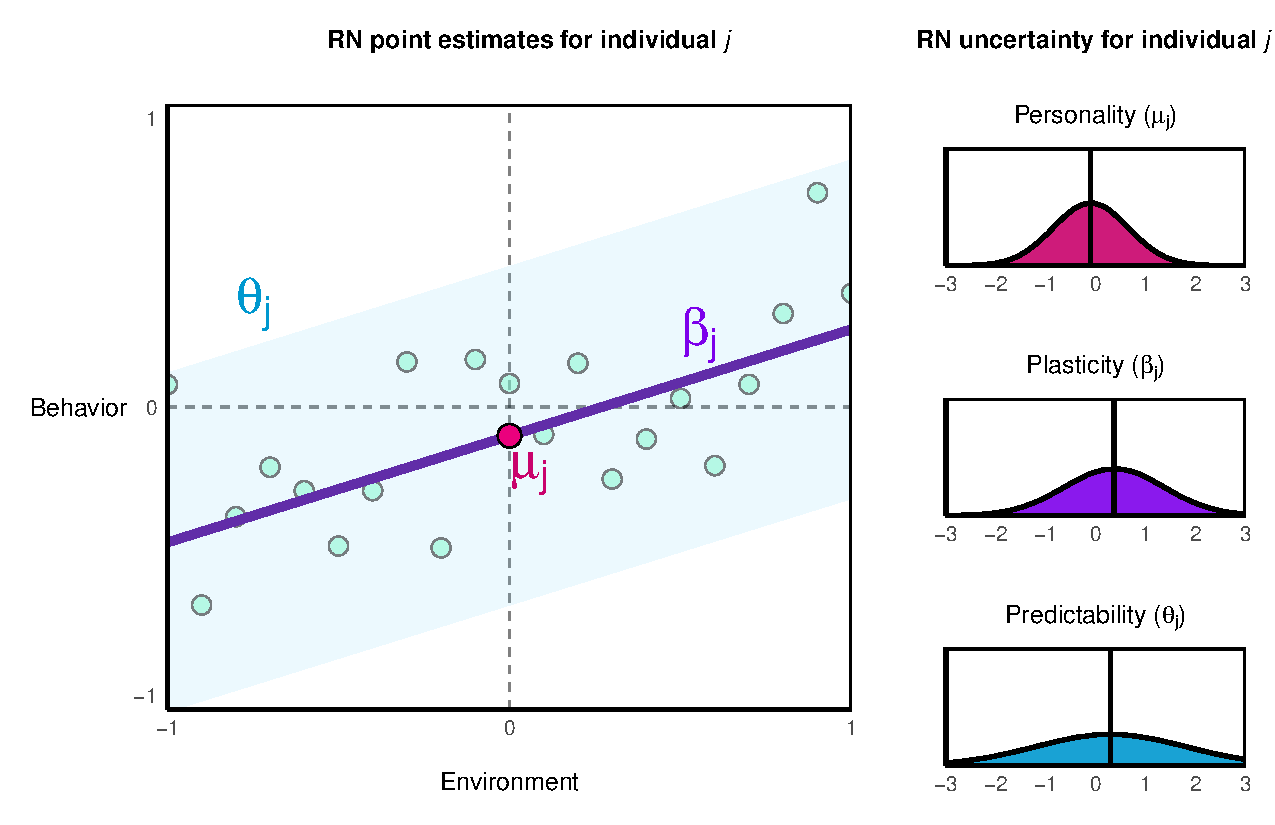
\includegraphics[scale=0.8]{fig1.pdf}
\caption{A behavioral reaction norm (RN) for individual $j$ defined across an environmental gradient. The individual's reaction norm is defined by three parameters indicated in the left plot: (i) the RN intercept trait value $\mu_j$ describing behavioral consistency (i.e. personality) across environments; (ii) the RN slope trait value $\beta_j$ capturing behavioral plasticity across environments; and (iii) the RN dispersion trait value $\theta_j$ reflecting behavioral predictability across environments, as indicated by the $95\%$ shaded credible interval (i.e. $\pm 1.96*\theta_j$).  Individuals' true RN parameters will be unknown in empirical research and must be inferred from raw longitudinal measurements (teal circles) across the environmental gradient. These inferences will generally be subject to high degrees of statistical uncertainty, as captured by the posterior distributions of each RN parameter shown on the right. RN point estimates (BLUPs) taken from these posterior distributions, such as the mean values indicated by the black vertical lines, ignore this uncertainty and provide misleading confidence in the shape of an individuals' behavioral strategy. For example, it can be seen that there is a wide range of possible values for individual $j$'s parameters with similar degrees of posterior support, particularly for the highly uncertain predictability trait value. As has been previously emphasized in the literature, failure to account for this uncertainty around point estimates can lead to anti-conservative inference and an increased risk of false positives. See the main text for further discussion.}
\label{fig:fig1}
\end{figure}

\hypertarget{current-approaches}{%
\section{Current approaches}\label{current-approaches}}

The basic challenge of modelling RN effects is to effectively account
for the uncertainty in RN parameters (i.e.~BLUPs) across all stages of
analysis. Variation in phenotypes with low to moderate repeatability is,
by definition, largely explained by factors other than
between-individual differences. As a consequence, sampling designs with
modest repeated measurements and uncontrolled environmental variation
typically result in highly uncertain estimation of RNs. Failure to
account for the uncertainty of RNs across subsequent stages of analysis
artificially reduces uncertainty in the inferred effects of RNs, as
uncertainty in individuals' trait values necessarily translates into
uncertainty about the effects of these trait values, and can thus
undesirably increase the risk of false positives. For this reason,
\protect\hyperlink{ref-Hadfield2010}{Hadfield et al.}
(\protect\hyperlink{ref-Hadfield2010}{2010}) discouraged all future use
of BLUP point estimates in evolutionary ecology, so as to prevent the
proliferation of misleading findings in the literature. Nevertheless,
because the theoretical significance of RNs is not diminished by the
difficulty of appropriately modeling their effects, many behavioral
ecologists without clear alternative solutions continued to misuse point
estimates of BLUPs in their research. In response,
\protect\hyperlink{ref-Hous2017}{Houslay and Wilson}
(\protect\hyperlink{ref-Hous2017}{2017}) provided a detailed overview of
appropriate strategies for tackling this challenge, emphasizing that
multivariate GLMMs with covarying random effects can be used to
effectively account for uncertainty in RNs across multiple response
models. Despite these repeated cautionary notes, some researchers still
continue to utilize BLUP point estimates (e.g.
\protect\hyperlink{ref-Ding2020b}{Dingemanse et al. 2020}) or raw data
(e.g. \protect\hyperlink{ref-Brehm2019}{Brehm et al. 2019}) for testing
RN effects, even while acknowledging the work of
\protect\hyperlink{ref-Hadfield2010}{Hadfield et al.}
(\protect\hyperlink{ref-Hadfield2010}{2010}) and
\protect\hyperlink{ref-Hous2017}{Houslay and Wilson}
(\protect\hyperlink{ref-Hous2017}{2017}). This likely reflects the fact
that the random effects models proposed by
\protect\hyperlink{ref-Hous2017}{Houslay and Wilson}
(\protect\hyperlink{ref-Hous2017}{2017}) do not readily extend to a
variety of more complex RN effects that cannot be straightforwardly
derived from random effect covariances and correlations. This section
briefly reviews current solutions for the misuse of BLUPs and discusses
their benefits and limitations.

\hypertarget{multivariate-glmms-with-covarying-random-effects}{%
\subsection{Multivariate GLMMs with covarying random
effects}\label{multivariate-glmms-with-covarying-random-effects}}

Popular GLMM software such as the ``lme4'' R package
(\protect\hyperlink{ref-Bates2014}{Bates et al. 2014}) do not readily
address multivariate, integrated phenotypes. As a consequence,
researchers are often motivated to (i) estimate RNs from a univariate
response model of a relevant behavior, and (ii) subsequently enter BLUP
point estimates of these RNs as covariates in another response model.
Fortunately, the risk engendered by this approach can be readily
overcome by specifying a multivariate GLMM that simultaneously accounts
for uncertainty in behavioral BLUPs and their associations with other
responses. \protect\hyperlink{ref-Hous2017}{Houslay and Wilson}
(\protect\hyperlink{ref-Hous2017}{2017}) demonstrate how this can be
accomplished with random effect correlations or covariances for
phenotypic and quantitative genetic studies, using both frequentist and
Bayesian software.

The multivariate GLMMs proposed by
\protect\hyperlink{ref-Hous2017}{Houslay and Wilson}
(\protect\hyperlink{ref-Hous2017}{2017}) are an extremely valuable tool
for behavioral ecologists interested in RNs and integrated phenotypes.
These models provide desirable flexibility for addressing a variety of
questions beyond simply quantifying random effect variances and
covariances, although this is on its own quite an important task. As any
student of multivariate statistics is well aware, trait covariance
matrices can be readily transformed to provide a veritable treasure
chest of biological insights (\protect\hyperlink{ref-Blows2007}{Blows
2007}), such as identifying trajectories of phenotypic conservation and
divergence among closely related populations
(\protect\hyperlink{ref-Roy2020}{Royauté, Hedrick, and Dochtermann
2020}), discovering latent behavioral characters and networks causing
covariance among multiple traits
(\protect\hyperlink{ref-Araya2014}{Araya-Ajoy and Dingemanse 2014};
\protect\hyperlink{ref-Martin2019}{Martin et al. 2019}), and calculating
linear selection differentials and genetic responses to selection
(\protect\hyperlink{ref-Stinch2014}{Stinchcombe, Simonsen, and Blows
2014}). Thus, this method can be used to accomplish many empirical goals
with relative ease.

Nevertheless, there are important cases where further information is
desired that cannot be derived from random effect covariation alone,
limiting the utility of these models for explaining the effects of RNs
on evolutionarily relevant outcomes. This is why fixed effects remain
important for testing evolutionary ecological theory, because we often
want to directly parameterize specific functional relationships between
traits, as well as to specify the direction of these effects. In other
words, we often want to know whether a behavior affects another measure
in a specific, potentially nonlinear manner, and perhaps in interaction
with other traits or states, rather than merely asking whether the trait
and the outcome are linearly associated through any number of possible
causal pathways in either direction. This issue is not specific to the
models proposed by \protect\hyperlink{ref-Hous2017}{Houslay and Wilson}
(\protect\hyperlink{ref-Hous2017}{2017}), but is rather a limitation of
variance-partitioning models more generally, which tend to trade off
explanatory power and causal insight for accurate description and
\emph{in situ} prediction (\protect\hyperlink{ref-Briley2019}{Briley et
al. 2019}; \protect\hyperlink{ref-Hadfield2017}{Hadfield and Thomson
2017}; \protect\hyperlink{ref-Okasha2020}{Okasha and Otsuka 2020}).

A particular concern is that testing adaptive theory of individual
variation often requires evaluating nonlinear selection on behavioral
RNs (\textbf{Figure \ref{fig:fig2}}). In general, these nonlinear
effects cannot be accurately estimated by random effect covariances, as
covariance is by definition a measure of linear dependency and thus does
not capture nonlinear dependencies among measures. However, it is
straightforward to capture these patterns using fixed quadratic and
interaction effects in a parametric fitness model
(\protect\hyperlink{ref-Lande1983}{Lande and Arnold 1983}). For example,
if the population RN is at an evolutionary equilibrium, so that RN
variation is non-adaptive within the population and results from
processes such as mutation-selection balance or developmental noise
(e.g. \protect\hyperlink{ref-Bierbach2017}{Bierbach, Laskowski, and Wolf
2017}; \protect\hyperlink{ref-Tooby1990}{Tooby and Cosmides 1990}), then
we should expect to find evidence of stabilizing selection around the
population average RN parameters. In the absence of correlational
selection, this would be observed in a Lande-Arnold selection analysis
as null or weak linear effects and negative quadratic effects
(\protect\hyperlink{ref-Stinch2008}{Stinchcombe et al. 2008}), assuming
the population had not been recently displaced from a fitness peak by
non-adaptive processes. Alternatively, strong disruptive selection,
potentially indicative of ongoing behaviorally-mediated speciation
(\protect\hyperlink{ref-Wolf2012}{Wolf and Weissing 2012}), would be
expected to surface as the opposite pattern--null or weak linear effects
with positive quadratic effects.

When individual variation is adaptive and maintained through balancing
selection caused by spatially and/or temporally varying fitness effects
(e.g. \protect\hyperlink{ref-Gurven2014}{Gurven et al. 2014}; Le
\protect\hyperlink{ref-LC2015}{Cœur et al. 2015}), interaction effects
will be expected between local ecological conditions (e.g.~season,
population density, resource abundance) and individuals' RN parameters
(\protect\hyperlink{ref-Wright2019}{Wright et al. 2019}). Similar
considerations apply to social contexts addressed by evolutionary game
theory, in which frequency-dependent fitness functions, such as
cooperative strategies with diminishing returns or threshold effects as
a function of partners' strategies
(\protect\hyperlink{ref-McNamara2020}{McNamara and Leimar 2020}), will
be observed through interactive selection effects
(\protect\hyperlink{ref-Araya2020}{Araya-Ajoy, Westneat, and Wright
2020}; \protect\hyperlink{ref-Martin2021}{Martin and Jaeggi 2021};
\protect\hyperlink{ref-Queller2011}{Queller 2011}). When adaptive
individual variation is maintained through state-dependent calibration
or feedback processes (e.g.~von
\protect\hyperlink{ref-Rueden2015}{Rueden, Lukaszewski, and Gurven
2015}; \protect\hyperlink{ref-Sih2015}{Sih et al. 2015}), then
phenotypes should also interact with state variables to determine
fitness outcomes. Adaptive behavioral syndromes may further evolve
through correlational selection for specific RN parameter combinations.
Cichlid \emph{Pelvicachromis pulcher} females' mating preferences, for
example, select for males with high levels of both personality and
predictability in aggressiveness
(\protect\hyperlink{ref-Scherer2018}{Scherer, Kuhnhardt, and Schuett
2018}). When RNs are under such correlational selection, interaction
effects are expected between RN parameters on fitness
(\protect\hyperlink{ref-Blows2003}{Blows 2003}). Of course, these
considerations also apply to a host of RN effects on outcomes other than
fitness, such as the exponential effects of personality in activity
level and anxiety on seed removal and dispersal among small mammals
(\protect\hyperlink{ref-Brehm2019}{Brehm et al. 2019}). In all such
cases, one would not detect these theoretically pertinent relationships
using linear covariances among random effects, but must instead directly
specify fixed quadratic and interactive effects caused by behavioral
RNs. A variety of more complex fitness surfaces can also be captured
through the combination of these quadratic and interaction effects
(\protect\hyperlink{ref-Phillips1989}{Phillips and Arnold 1989}), or
higher term polynomials, as shown in \textbf{Figure \ref{fig:fig2}} for
a bivariate analysis.

A potential solution to this challenge is to model the squared and
product values of raw measurements as additional responses with
covarying random effects, which can subsequently be used to calculate
nonlinear selection gradients
(\protect\hyperlink{ref-Ding2021}{Dingemanse, Araya‐Ajoy, and Westneat
2021}). However, this approach does not differentiate between the
fitness effects of personality, plasticity, and predictability, and it
does not appropriately partition between- and within-individual
(co)variation in non-Gaussian measurements. To calculate nonlinear
selection gradients for non-Gaussian responses, expected trait values
should be first estimated on a latent linear scale, through the use of
an appropriate GLMM link function, before being squared or multiplied
together. This ensures that nonlinear mean and variance effects are
correctly predicted on the original data scale
(\protect\hyperlink{ref-Nelder1972}{Nelder and Wedderburn 1972}).

\hypertarget{two-stage-analyses}{%
\subsection{Two-stage analyses}\label{two-stage-analyses}}

Another solution to the challenges posed by the random effects method is
to instead (i) estimate BLUP posteriors in a Bayesian random effects
model, and then (ii) estimate a separate model with fixed RN effects,
running the analysis repeatedly over the posterior distribution of BLUPs
estimated in the first model. While this approach technically carries
the uncertainty in RNs forward, thus avoiding the undesirable
consequences of point estimates, it can nevertheless result in
downwardly biased estimates of the RN fixed effects, as
\protect\hyperlink{ref-Ding2020b}{Dingemanse et al.}
(\protect\hyperlink{ref-Ding2020b}{2020}) observed in supplementary
simulations. Although these authors did not provide an explanation for
the observed bias, it can be attributed to a more general statistical
phenomenon known as attenuation bias, in which independent measurement
error in a predictor variable causes downward bias in its association
with an outcome measure (\protect\hyperlink{ref-Adolf2007}{Adolph and
Hardin 2007}; \protect\hyperlink{ref-Spearman1904}{Spearman 1904}). This
is caused by the BLUPs in the initial model being estimated
independently of the RN effects on the outcome of interest, so that the
estimated uncertainty in BLUPs is by design statistically independent of
uncertainty in the RN effects estimated in the second stage of the
analysis. This does not, however, make the use of BLUP point estimates
any less risky or more desirable, but is simply an artifact of not
simultaneously accounting for both sources of uncertainty in the same
model. It is important to remember that BLUPs and RNs are latent,
statistical inferences, not directly measured trait values or mere
averages of raw trait values, and as such are particularly sensitive to
correct model specification
(\protect\hyperlink{ref-Hadfield2010}{Hadfield et al. 2010};
\protect\hyperlink{ref-Postma2006}{Postma 2006}). A related alternative
solution is to handle attenuation bias by adjusting selection
coefficients on raw trait values with repeatability estimates, rather
than directly using BLUPs in the fitness model
(\protect\hyperlink{ref-Ding2021}{Dingemanse, Araya‐Ajoy, and Westneat
2021}). However, this approach does not provide a means of
differentiating nonlinear selection on personality, plasticity and
predictability, nor does it generalize to non-Gaussian measurements
where repeatability is best expressed on a transformed linear scale due
to non-linear mean and variance effects on the original scale.

\begin{figure}
\hspace*{-1.75cm}
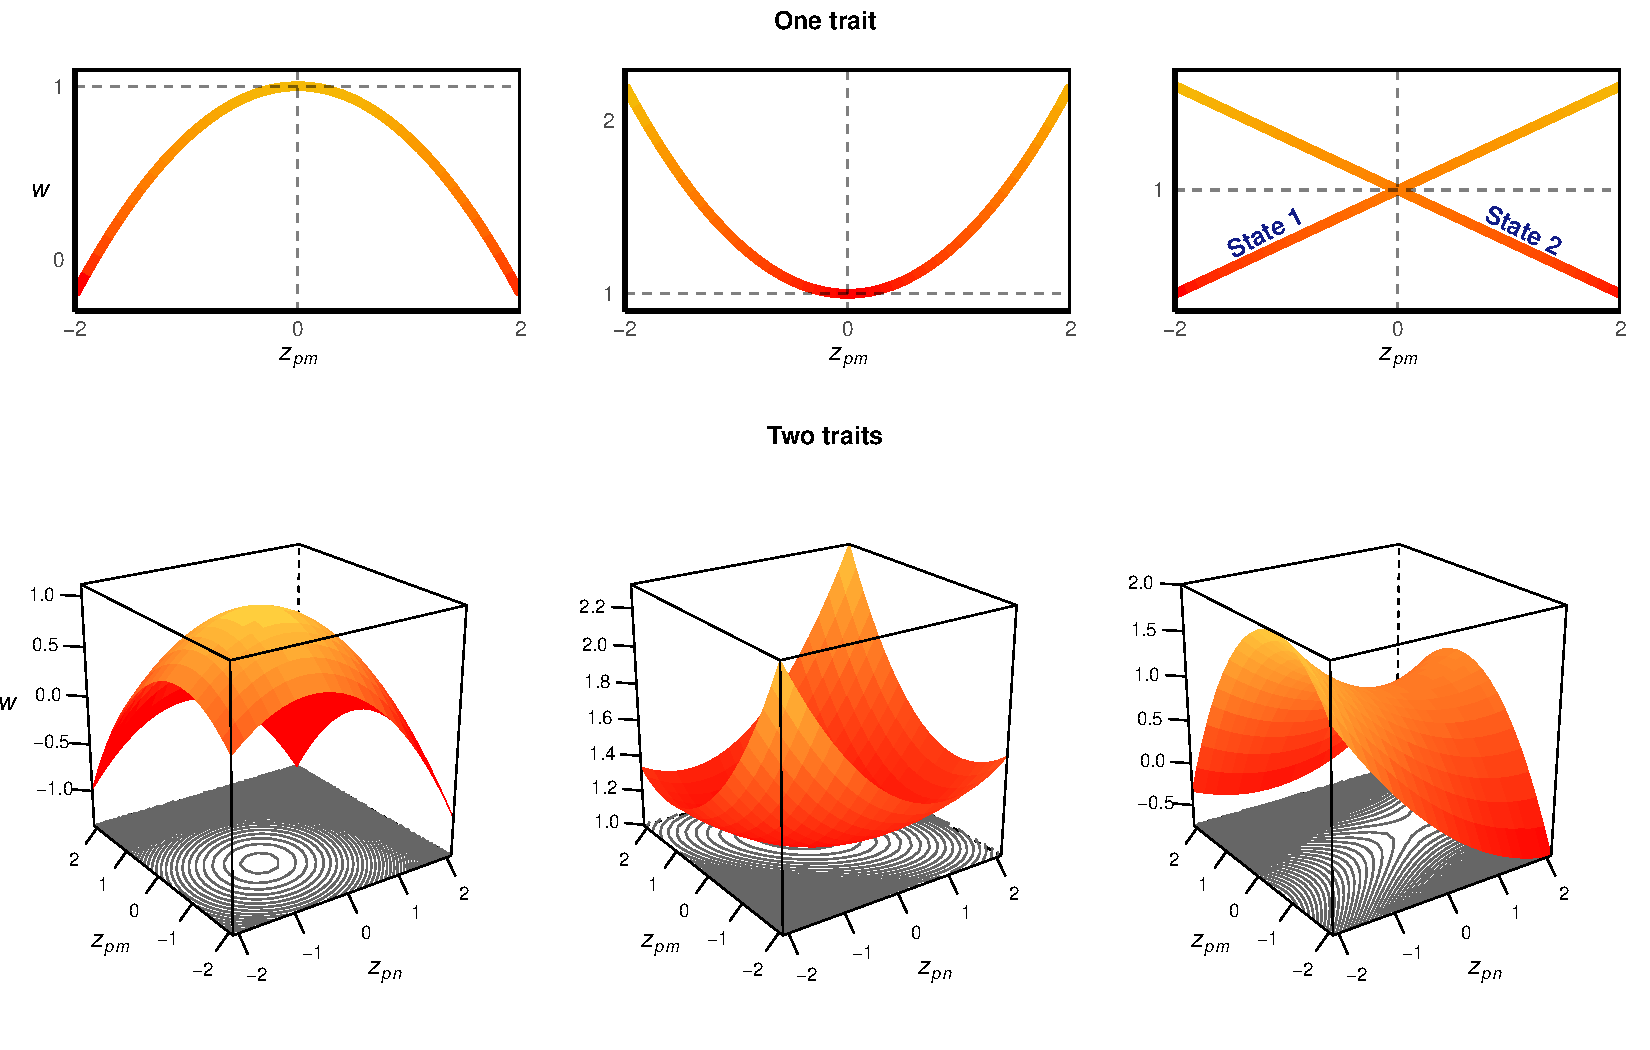
\includegraphics[scale=0.7]{fig2.pdf}
\caption{Nonlinear selection surfaces for behavioral RNs. Adaptiveness is indicated by the color of the line or surface, with red indicating lower relative fitness ($w$) and gold indicating higher relative fitness. \\ \\
$\boldsymbol{Top \ row}$. Patterns of nonlinear selection on a single behavioral RN parameter ${z_{\mathrm{p}m}}$, which also apply to selection on multiple traits in the absence of correlational selection between traits. Dashed lines intercept the expected population-level trait value and relative fitness at (${z_{\mathrm{p}m}}=0, {w}=1$). $Left \ panel$: stabilizing selection on trait values, which maintains the population average trait value at an evolutionary equilibrium and reduces individual variation. $Middle \ panel$: disruptive selection, which increases the frequency of extreme trait values and increases individual variation as a consequence. $Right \ panel$: balancing selection, in which the fitness consequences of a trait value vary across different states, causing the maintenance of individual variation across multiple selection events. States refer to any factors that modulate the fitness consequences of a behavior, such as differing spatial and/or temporal contexts, population densities, or frequencies of social partner strategies. States may also be endogenous factors that determine whether it is adaptive to express a particular RN trait value, such as the effects of body size and condition on the fitness consequences of boldness and aggression.  \\ \\
$\boldsymbol{Bottom \ row}$. Patterns of nonlinear selection on two behavioral RN parameters ${z_{\mathrm{p}m}}$ and ${z_{\mathrm{p}n}}$. Due to the presence of correlational selection, the adaptiveness of any trait value for parameter $m$ is contingent on the trait value for parameter $n$ (and vice versa). $Left \ panel$: a dome-shaped selection surface, where a combination of slightly negative parameters has the highest fitness. $Middle \ panel$: a bowl-shaped selection surface, with the most adaptive phenotypes combining extremely high or low trait values in both parameters. $Right \ panel$: a saddle-shaped selection surface, where phenotypes combining moderate trait values for $m$ and extremely low trait values for $n$ achieve the highest relative fitness.
}
\label{fig:fig2}
\end{figure}

\hypertarget{a-novel-solution}{%
\section{A novel solution}\label{a-novel-solution}}

Given the limitations of relying solely on covarying random effects,
behavioral ecologists stand to benefit from adding an additional
modeling approach to their toolkit, one capable of directly estimating
nonlinear RN effects of arbitrary complexity. Here I propose a novel
solution that is a straightforward extension of
\protect\hyperlink{ref-Hous2017}{Houslay and Wilson}
(\protect\hyperlink{ref-Hous2017}{2017}) `s previous work: Bayesian
multi-response GLMMs in which individuals' RNs are simultaneously
treated as random effects on their observed behaviors as well as fixed
effects on outcome measures of interest (e.g.~survival and reproduction,
habitat choice, performance in an experimental task, etc.). In this
section, this basic modelling approach is formally introduced, along
with various extensions of interest for specific empirical scenarios. I
also end by proposing a novel and straightforward method for visualizing
the within-generation effects of multivariate selection on reaction
norms.

\hypertarget{multivariate-glmms-for-nonlinear-selection-on-rns}{%
\subsection{Multivariate GLMMs for nonlinear selection on
RNs}\label{multivariate-glmms-for-nonlinear-selection-on-rns}}

Our goal in overcoming the limitations of previous approaches is to
specify a GLMM with one response model estimating RN parameters of a
relevant behavior, as well as another response model that estimates the
effects of these RN parameters on a fitness-relevant measure. To enhance
comprehension, the RN response model is first considered in isolation
before being integrated into a single multi-response model below.

\hypertarget{reaction-norm-response-model}{%
\subsubsection{Reaction norm response
model}\label{reaction-norm-response-model}}

To model the RN parameters \(\boldsymbol{z_{\mathrm{p}}}\) for a
repeatedly measured behavior \(\boldsymbol{z}\) across an environmental
gradient \(\boldsymbol{x}\), we specify a GLMM for observation \(i\) of
individual \(j\) such that \begin{equation} \tag{1.1}\label{eq:1.1}
\begin{gathered}[t]
z_{ij} \sim f \left(\eta_{ij}, \theta_{ij} \right)  \\
g_\eta \left( \eta_{ij} \right) = \mu_0 + \mu_j + \left(\beta_1 + \beta_j \right) x_{ij} \nonumber \\
g_\theta \left( \theta_{ij} \right) = \theta_0 + \theta_{j} \nonumber \\
 \boldsymbol{z_{\mathrm{p}}}= \begin{bmatrix}
\boldsymbol{\mu} &
\boldsymbol{\beta} &
\boldsymbol{\theta} \end{bmatrix} ^{\prime}
\sim \mathrm{M}\mathrm{VNormal} \left(
\boldsymbol{0},\boldsymbol{\mathrm{P}} \right) \nonumber \\ 
\end{gathered}
\end{equation} Bold values are used to distinguish vectors and matrices
from scalars and primes \(\prime\) are used to indicate the transpose
operation. Individuals' traits values are specified as being generated
by some probability density function \(f\) with corresponding location
\(\boldsymbol{\eta}\) and dispersion \(\boldsymbol{\theta}\) parameters,
such as the means and standard deviations of normal distributions or the
means and shape parameters of gamma, negative binomial, and beta
distributions. For GLMMs, these nonlinear parameters are modelled on a
latent linear scale using link functions \(g_{\eta}\) and \(g_{\theta}\)
(e.g.~identity, log, logistic, or reciprocal transformations). We
therefore refer to \(g_{\eta}(\eta_{ij})\) and
\(g_{\theta}(\theta_{ij})\) as the linear predictors for the respective
location and dispersion parameters of observation \emph{i} on individual
\emph{j}.

Typically, personality and plasticity are modelled through the linear
predictor of the location parameters, capturing variation in expected
behavior (i.e.~predicted behavior averaged over dispersion). This is
accomplished through the estimation of random intercept \(\mu_j\) and
random slope \(\beta_j\) for individual \(j\), which are expressed as
deviations from the population-average intercept \(\mu_0\) and slope
\(\beta_1\). These parameters correspond to the elevation and slope of
the individual's behavioral RN. We assume that environmental exposures
are randomized across individuals, so that there is no need to
within-individual center the covariate used for scaling RN slopes (van
de \protect\hyperlink{ref-Pol2009}{Pol and Wright 2009}). Predictability
is modelled through a random intercept effect \(\theta_j\) on the
dispersion parameters, deviating from the population-average dispersion
\(\theta_0\), which captures individual-specific variability independent
of the linear predictor. The effect of each parameter in
\(\boldsymbol{z_{\mathrm{p}}}\) on the shape of an individual's RN can
be seen in \textbf{Figure \ref{fig:fig1}}. For simplicity, we ignore the
possibility that individuals may also exhibit plasticity in their
predictability as a function of the environment, although this could be
readily estimated, along with other fixed and random effects. For
distributions without an explicit dispersion parameter, such as Poisson
or binomial distributions, individual differences in predictability
cannot be directly modelled in this way. However, this limitation can be
easily avoided by using a closely related distribution accounting for
overdispersion, such as the negative binomial and beta binomial
distributions.

The associations among RN parameters are captured by the trait
covariance matrix \(\boldsymbol{\mathrm{P}}\). Note that covariance and
correlation matrices can always be translated to one another by
\(\boldsymbol{\mathrm{P}}=\boldsymbol{\mathrm{S}}\boldsymbol{\mathrm{R}}\boldsymbol{\mathrm{S}}\),
where \(\boldsymbol{\mathrm{S}}\) is a diagonal matrix with standard
deviations and \(\boldsymbol{\mathrm{R}}\) is a correlation matrix. This
identity is often useful for efficiently estimating Bayesian GLMMs by
separating out the scale and association parameters among random
effects. We therefore substitute
\(\boldsymbol{\mathrm{S}}\boldsymbol{\mathrm{R}}\boldsymbol{\mathrm{S}}\)
for \(\boldsymbol{\mathrm{P}}\) in subsequent formula.

\hypertarget{multi-response-model-for-selection-analysis}{%
\subsubsection{Multi-response model for selection
analysis}\label{multi-response-model-for-selection-analysis}}

Our goal is to now specify a single multi-response model that estimates
(Eq \ref{eq:1.1}) while also estimating the effects of RN parameters
\(\boldsymbol{z_{\mathrm{p}}}\) on fitness. Given that researchers will
often lack repeated measures of fitness or fitness-proxies (e.g.~bodily
condition, clutch size, mate choice), the presented models assume that a
single fitness measure is available per individual, although this
assumption can be relaxed by including additional random effects to
account for unobserved heterogeneity in repeated fitness measures. For
simplicity, we also begin by assuming that the fitness measure can be
effectively described by a Gaussian distribution, which simplifies the
estimation of selection gradients and differentials below. As is
appropriate for modelling relative fitness
(\protect\hyperlink{ref-Lande1983}{Lande and Arnold 1983}), \(w\) is
mean-scaled so that \(w_j = W_j/\bar{W}\) where \(\bar{W}\) is the mean
absolute fitness across individuals. For notational clarity, we now
introduce superscripts \((z)\) to distinguish parameters that are
specific to the \(z\) behavioral response model from those in the \(w\)
fitness response model.

\begin{equation} \tag{1.2}\label{eq:1.2}
\begin{gathered}[t]
z_{ij} \sim f \left(\eta^{(z)}_{ij }, \theta^{(z)}_{ij} \right)  \\
g_\eta \left( \eta^{(z)}_{ij} \right) = \mu_0^{(z)} + \mu_j^{(z)}+ \left(\beta_1^{(z)} + \beta_j^{(z)} \right) x_{ij} \nonumber \\
g_\theta \left( \theta^{(z)}_{ij} \right) = \theta_0^{(z)} + \theta_{j}^{(z)} \nonumber \\
\boldsymbol{z_{\mathrm{p}}} = \begin{bmatrix}
\boldsymbol{\mu}^{(z)} &
\boldsymbol{\beta}^{(z)} &
\boldsymbol{\theta}^{(z)} \end{bmatrix} ^{\prime}
 \sim \mathrm{M}\mathrm{VNormal} \left(
\boldsymbol{0},\boldsymbol{\mathrm{S}}\boldsymbol{\mathrm{R}}\boldsymbol{\mathrm{S}} \right) \nonumber \\ 
\nonumber \\
w_{j} \sim \mathrm{Normal} \left( \mu_{j}, \sigma _{j} \right) \nonumber \\
\mu _{j} = \mu_0 + \beta_1 \left( \mu^{(z)}_{j} \right) + 
                \beta_2 \left( \beta_j^{(z)} \right) + 
                \beta_3 \left( \theta^{(z)}_{j} \right)  \nonumber  \\ 
                + \beta_4 \left( \mu^{(z)}_j \mu^{(z)}_j \right) +
                \beta_5\left( \beta^{(z)}_j \beta^{(z)}_j \right) +
                \beta_6 \left( \theta^{(z)}_j \theta^{(z)}_j \right)\\ 
                +  \beta_7 \left( \mu^{(z)}_j \beta^{(z)}_j \right) + 
                \beta_8 \left( \mu^{(z)}_j \theta^{(z)}_j \right) + 
                 \beta_9 \left( \beta^{(z)}_j \theta^{(z)}_j \right) \nonumber \\ 
\end{gathered}
\end{equation}

Readers familiar with structural equation modelling
(\protect\hyperlink{ref-Araya2014}{Araya-Ajoy and Dingemanse 2014};
\protect\hyperlink{ref-Martin2019}{Martin et al. 2019}) may note that
each RN parameter in this model can be conceptualized as an exogenous
latent variable, with its loading on trait \(z\) fixed to 1, thus
scaling the zero-centered latent variable, and its loadings on trait
\(w\) estimated with the regression coefficients. These latent variables
separate out the portions of variance in trait \(\boldsymbol{z}\) due to
each latent RN parameter and, therefore, isolate distinct RN effects on
fitness from all other sources of non-repeatable variation in the raw
trait values. The proposed model can also be conceptualized as an
extension of the so-called `errors-in-variables' models discussed by
\protect\hyperlink{ref-Ding2021}{Dingemanse, Araya‐Ajoy, and Westneat}
(\protect\hyperlink{ref-Ding2021}{2021}), which do not disentangle
repeatable variation in raw measurements due to personality, plasticity,
and predictability. This multi-response GLMM thus provides a flexible
and intuitive means of integrating the benefits as well as overcoming
the limitations of multiple previously suggested statistical approaches.
It is also important to note that the proposed model can always be
simplified to facilitate studies of selection on individual RN
parameters, should researchers lack sufficient repeated samples or
environmental data to simultaneously address personality, plasticity,
and predictability.

When this quadratic regression model effectively approximates the
individual selection surface (\protect\hyperlink{ref-Lande1983}{Lande
and Arnold 1983}; \protect\hyperlink{ref-Phillips1989}{Phillips and
Arnold 1989}),
\(\boldsymbol{\upbeta}=\left[\beta_1,\beta_2,\beta_3 \right]\) indicates
the expected direction and magnitude of unconstrained adaptation in the
average population RN values, which are also known as directional
selection gradients. Nonlinear effects are instead captured by
\(\upgamma _{\mu,\mu}=\beta_4*2, \ \upgamma _{\beta,\beta}= \beta_5*2,\)
and \(\upgamma _{\theta,\theta}= \beta_6*2\), which indicate convex or
concave curvature in the selection surfaces of RN parameters
(\protect\hyperlink{ref-Stinch2008}{Stinchcombe et al. 2008}), and
\(\upgamma _{\mu,\beta}=\beta_7, \ \upgamma _{\mu,\theta}=\beta_8,\) and
\(\upgamma _{\beta,\theta}=\beta_9\), which indicate further curvature
due to the presence of correlational selection between trait pairs. The
regression coefficients capturing nonlinear curvature in the selection
surface can then be grouped into a matrix \(\boldsymbol{\upgamma}\) of
quadratic selection gradients and the fitness model can be simplified to
matrix notation for individual \(j\) such that

\begin{equation} \tag{1.3}\label{eq:1.3}
\begin{gathered}[t]
\mu_{j} = \mu_0 + \boldsymbol{\upbeta}^{{\prime}}\boldsymbol{z}_{\boldsymbol{\mathrm{p}}j} + \boldsymbol{z}^{\prime}_{\boldsymbol{\mathrm{p}}j} \boldsymbol{\upgamma} \boldsymbol{z}_{\boldsymbol{\mathrm{p}}j} \\
\boldsymbol{\mathrm{\upgamma}} =
\begin{pmatrix}
\upgamma _{\mu,\mu} & 
\upgamma _{\mu,\beta} &
\upgamma _{\mu,\theta} \\
\upgamma _{\beta,\mu} & \upgamma _{\beta,\beta} & \upgamma _{\beta,\theta} \\
\upgamma _{\theta,\mu} & \upgamma _{\theta,\beta} & \upgamma _{\theta,\theta} 
\end{pmatrix} \nonumber
\end{gathered}
\end{equation}

If one desires to express gradients in standardized units for effect
size comparison, then
\(\boldsymbol{z}^*_{\boldsymbol{\mathrm{p}}j}=\boldsymbol{z}_{\boldsymbol{\mathrm{p}}j}\oslash \mathrm{diag}(\boldsymbol{\mathrm{S}})\)
can instead be specified in the fitness response model, where the
Hadamard division \(\oslash\) indicates element-wise division of each
parameter by its standard deviation, which are contained on the diagonal
of the \(\boldsymbol{\mathrm{S}}\) matrix. The selection model can also
be extended to account for various kinds of balancing selection (see
\textbf{Figure \ref{fig:fig2}}) by including additional interaction
effects for the relevant state variables. For example,
\(\beta_{I} ( \mu^{(z)}_{j} * \mathrm{N} )\) could be estimated to
assess the presence of density-dependent selection on personality across
differing population sizes \(\mathrm{N}\).

It is common in selection analyses to estimate linear and nonlinear
gradients on observed trait values \(\boldsymbol{z}\), rather than
directly on RN parameters \(\boldsymbol{z}_{\boldsymbol{\mathrm{p}}}\)
as proposed here. However, it is ultimately the repeatable individual
variation in a phenotype that is available to selection, with all other
trait variation effectively representing measurement error from the
perspective of evolutionary inference at the population level
(\protect\hyperlink{ref-Martin2021}{Martin and Jaeggi 2021}). Thus, it
is genetically encoded behavioral strategies (i.e.~RNs) that are adapted
within a population, rather than the specific actions animals are
observed taking in any particular measurement context
(\protect\hyperlink{ref-McNamara2020}{McNamara and Leimar 2020}).
Moreover, when RN parameters are not completely integrated, so that
\(\boldsymbol{\mathrm{R}} \neq \boldsymbol{1}\), selection can further
act on independent variation in each element of
\(\boldsymbol{z}_{\boldsymbol{\mathrm{p}}}\), leading to distinct
changes in the population RN intercept, slope, and dispersion within and
across generations. These adaptive processes will be confounded when
solely considering selection on observed trait values
\(\boldsymbol{z}\). The global effects of RN parameter selection on the
shape of the population RN function can also be straightforwardly
estimated and visualized using methods developed further below.

\hypertarget{fully-bayesian-inference}{%
\subsubsection{Fully Bayesian
inference}\label{fully-bayesian-inference}}

To the best knowledge of the author, the proposed multi-response model
for RN selection analysis cannot be straightforwardly estimated with
mainstream statistical software. This does not, however, reflect any
fundamental issue with its parameterization or interpretation, but
rather pragmatic limitations of the estimators and/or syntax used in
these software, which generally do not allow the same latent parameters
to be specified across different GLMM response models. Fortunately, the
Stan statistical programming language
(\protect\hyperlink{ref-Stan}{Carpenter et al. 2017}), which relies on
cutting-edge and computationally efficient Markov Chain Monte Carlo
(MCMC) algorithms, provides exceptional flexibility for specifying and
straightforwardly estimating such atypical GLMMs within a Bayesian
framework. Researchers unfamiliar with the general benefits of fully
Bayesian inference are encouraged to see
\protect\hyperlink{ref-Rethinking}{McElreath}
(\protect\hyperlink{ref-Rethinking}{2020}) for detailed discussion, as
well as \protect\hyperlink{ref-Gelman2020}{Gelman et al.}
(\protect\hyperlink{ref-Gelman2020}{2020}) for helpful tips on
developing an effective Bayesian workflow for data analysis. A brief
review of some fundamentals will facilitate robust estimation and
hypothesis testing with the proposed model.

To estimate Eq \ref{eq:1.2} within a Bayesian framework, we simply need
to specify prior distributions for all the population-level parameters,
which are transformed within the model to derive the individual-level RN
parameters during model estimation. \begin{align*}
\mu_0^{(z)},\beta_1^{(z)}, \theta_0^{(z)}, \boldsymbol{\mathrm{S}}, \boldsymbol{\mathrm{R}}, \mu_0, \sigma, \beta_1, ... , \beta_9
\sim \boldsymbol{f}(\boldsymbol{\Phi})
\end{align*}

As above, \(\boldsymbol{f}\) are probability density functions for each
parameter and \(\boldsymbol{\Phi}\) are the corresponding distributional
parameters for all priors. Although it is common for ecology methods
papers to use and/or recommend using highly diffuse or flat priors (e.g.
\protect\hyperlink{ref-Hous2017}{Houslay and Wilson 2017};
\protect\hyperlink{ref-Vill2016}{Villemereuil et al. 2016}), it is also
well established within the statistics literature that weakly
informative, regularizing priors--which slightly pull parameters toward
null values and provide low prior probability to extreme effect
sizes--facilitate more robust inferences and should generally be
preferred over flat priors whenever possible
(\protect\hyperlink{ref-Gelman2000}{Gelman and Tuerlinckx 2000};
\protect\hyperlink{ref-Rethinking}{McElreath 2020};
\protect\hyperlink{ref-Lemoine2019}{Lemoine 2019}). This does not
require that one has access to a relevant meta-analysis or is in a
position to make strong a priori assumptions about the true effect size
(cf. \protect\hyperlink{ref-Ellison2004}{Ellison 2004}). Rather, one can
simply use general-purpose, conservative priors as a means of increasing
the generalizability and robustness of their findings, even in a state
of relative ignorance about the true effect size. For most GLMMs, priors
such as \(\mu,\beta \sim \mathrm{Normal}(0,1)\),
\(\mathrm{diag}(\boldsymbol{\mathrm{S}}),\sigma \sim \mathrm{Exponential}(1)\),
and \(\boldsymbol{\mathrm{R}} \sim \mathrm{LKJ}(2)\) provide effective
weakly regularizing priors. See
\protect\hyperlink{ref-Lemoine2019}{Lemoine}
(\protect\hyperlink{ref-Lemoine2019}{2019}) for more detailed discussion
and recommendations in ecological research.

By specifying priors in the model, all parameters can subsequently be
estimated as posterior distributions. For example,
\(\boldsymbol{z}_{\boldsymbol{\mathrm{p}}}\) will no longer be estimated
with BLUP point estimates \(\hat{\mu}_j^{(z)}\),
\(\hat{\beta}_j^{(z)}\), and \(\hat{\theta}_j^{(z)}\), but will instead
be estimated with probability distributions capturing all of the
statistical uncertainty in the BLUPs \begin{align*}
\mathrm{Pr}\left( \mu_j^{(z)} \ | \ \boldsymbol{x},\boldsymbol{z},\boldsymbol{w},...,\boldsymbol{\Phi} \right), \quad
\mathrm{Pr}\left( \beta_j^{(z)} \ | \ \boldsymbol{x},\boldsymbol{z},\boldsymbol{w},...,\boldsymbol{\Phi} \right), \quad
\mathrm{Pr}\left( \theta_j^{(z)} \ | \ \boldsymbol{x},\boldsymbol{z},\boldsymbol{w},...,\boldsymbol{\Phi} \right)
\end{align*} These posterior distributions are conditional on the
observed measures (\(\boldsymbol{x},\boldsymbol{z},\boldsymbol{w}\)) and
all other model parameters and priors (\(...\boldsymbol{\Phi}\)). Given
that all statistical uncertainty is captured in these and other
posterior distributions, the proposed multi-response model (Eq
\ref{eq:1.2}) provides nearly unlimited flexibility for direct forms of
hypothesis testing. For example, to quantify our confidence that
positive correlational selection occurs for plasticity and
predictability, we simply need to manipulate the relevant posteriors to
calculate \begin{align*}
\mathrm{Pr}\left( \upgamma _ {\beta , \theta}  > 0 \ \mid \ \boldsymbol{x},\boldsymbol{z},\boldsymbol{w},...,\boldsymbol{\Phi} \right)
\end{align*} When posterior distributions are estimated with Markov
Chain Monte Carlo (MCMC), this value can be quantified by assessing this
inequality across the relevant vectors of posterior samples and
calculating the proportion of samples for which it is satisfied.
Similarly, if we want to quantify our confidence that there is stronger
directional selection on personality than plasticity, we can calculate
\begin{align*}
\mathrm{Pr}\left( \upbeta _ \mu  >  \upbeta _ \beta \ \mid \ \boldsymbol{x},\boldsymbol{z},\boldsymbol{w},...,\boldsymbol{\Phi} \right)
\end{align*} One could similarly perform a direct hypothesis test of a
more robust null hypothesis than is typically considered, given that
true effect sizes are almost never exactly zero in reality
(\protect\hyperlink{ref-Amrhein2019}{Amrhein, Trafimow, and Greenland
2019}; \protect\hyperlink{ref-Meehl1978}{Meehl 1978};
\protect\hyperlink{ref-Gelman2017}{Gelman and Carlin 2017}). Instead, a
direct test of a null hypothesis can provide the probability that an
effect is of a biologically trivial magnitude (e.g.~\textless{}
\textbar0.1\textbar{} for a standardized predictor). For instance,
considering the correlation among personality and predictability in the
\(\boldsymbol{\mathrm{R}}\) correlation matrix \begin{align*}
\mathrm{Pr}\left( -0.1 < \boldsymbol{\mathrm{R}}_{\mu, \theta}  < 0.1  \ \mid \ \boldsymbol{x},\boldsymbol{z},\boldsymbol{w},...,\boldsymbol{\Phi} \right)
\end{align*} Note that these tests are \emph{not} indirect null
hypothesis tests, which give the probability of observing the data under
the assumption that a null hypothesis is true. Instead, these are direct
tests of biologically substantive hypotheses given the observed data,
the evaluation of which is generally the primary goal of scientific
research. As such, intuitive interpretation can be made of the posterior
probabilities, so that values closer to 1 indicate greater support for
the tested hypotheses and values closer to 0 indicate stronger support
for the opposite hypotheses. These Bayesian hypothesis tests help to
avoid many common misinterpretations of classical tests, such as
interpreting confidence intervals as reflecting the probable range of
the true effect, interpreting \emph{P}-values as providing the
probability of the null hypothesis being true, or interpreting the
rejection of a null hypothesis test as being indicative of the
substantive (``alternative'') hypothesis being correct
(\protect\hyperlink{ref-Green2016}{Greenland et al. 2016};
\protect\hyperlink{ref-Rethinking}{McElreath 2020};
\protect\hyperlink{ref-McShane2019}{McShane et al. 2019}). Furthermore,
these Bayesian posteriors can be easily manipulated to address a variety
of questions which may not be easily specified directly in a statistical
model. This provides theoretically important benefits such as being able
to easily quantify uncertainty in and perform direct hypothesis tests on
derived quantities such as selection differentials, \(R^2\) values, and
repeatabilities.

\hypertarget{non-gaussian-fitness-measures}{%
\subsubsection{Non-Gaussian fitness
measures}\label{non-gaussian-fitness-measures}}

Despite the expected robustness of LMMs to violations of distributional
assumptions, any particular study will be at a non-trivial risk of
inferential bias when applying a linear fitness model to outcomes that
are clearly better described by a non-Gaussian distribution
(\protect\hyperlink{ref-Schiel2020}{Schielzeth et al. 2020}). Some
common non-Gaussian data types used for fitness-proxies include
dichotomous measures of survival or mating success, counts of offspring
fledged or surviving to adulthood, and various forms of zero-bounded
continuous performance measures such as growth rate or dispersal
distance. When considering RN effects on other biologically relevant
outcomes, there are of course a variety of non-Gaussian measures which
may be similarly employed, such as categorical, mutually exclusive
choices or reaction times in cognitive tasks, proportional measures of
time spent in an activity, and so on. In all such cases, researchers
will benefit from more reliable inferences and model predictions if they
try to accurately describe the data generating process with an
appropriate non-Gaussian distribution, rather than attempting to
pigeonhole their analysis into a linear model. Fortunately, the Stan
statistical programming language provides a plethora of possible
distributions for GLMM likelihood functions, as well as the capacity to
specify any custom likelihood functions of interest. To account for
non-Gaussian fitness measure \(W\), we update the fitness model in Eq
\ref{eq:1.2} with a generalized distributional function and link
transformation.

\begin{equation} \tag{2}\label{eq:2}
\begin{gathered}[t]
z_{ij} \sim f \left(\eta^{(z)}_{ij }, \theta^{(z)}_{ij} \right)  \\
g_\eta^{(z)} \left( \eta^{(z)}_{ij} \right) = \mu_0^{(z)} + \mu_j^{(z)}+ \left(\beta_1^{(z)} + \beta_j^{(z)} \right) x_{ij} \nonumber \\
g_\theta^{(z)} \left( \theta^{(z)}_{ij} \right) = \theta_0^{(z)} + \theta_{j}^{(z)} \nonumber \\
\boldsymbol{z_{\mathrm{p}}} = \begin{bmatrix}
\boldsymbol{\mu}^{(z)} &
\boldsymbol{\beta}^{(z)} &
\boldsymbol{\theta}^{(z)} \end{bmatrix} ^{\prime}
 \sim \mathrm{M}\mathrm{VNormal} \left(
\boldsymbol{0},\boldsymbol{\mathrm{S}}\boldsymbol{\mathrm{R}}\boldsymbol{\mathrm{S}} \right) \nonumber \\ 
\nonumber \\
W_{j} \sim f \left(\eta_{j}, \theta \right)   \nonumber \\
g_\eta \left( \eta_{j} \right)  = \mu_0 + \beta_1 \left( \mu^{(z)}_{j} \right) + 
                \beta_2 \left( \beta_j^{(z)} \right) + 
                \beta_3 \left( \theta^{(z)}_{j} \right)  \nonumber  \\ 
                + \beta_4 \left( \mu^{(z)}_j \mu^{(z)}_j \right) +
                \beta_5\left( \beta^{(z)}_j \beta^{(z)}_j \right) +
                \beta_6 \left( \theta^{(z)}_j \theta^{(z)}_j \right)\\ 
                +  \beta_7 \left( \mu^{(z)}_j \beta^{(z)}_j \right) + 
                \beta_8 \left( \mu^{(z)}_j \theta^{(z)}_j \right) + 
                 \beta_9 \left( \beta^{(z)}_j \theta^{(z)}_j \right) \nonumber \\ \nonumber \\ 
\mu_0^{(z)},\beta_1^{(z)}, \theta_0^{(z)}, \boldsymbol{\mathrm{S}}, \boldsymbol{\mathrm{R}}, \mu_0, \theta, \beta_1, ... , \beta_9
\sim \boldsymbol{f}(\boldsymbol{\Phi}) \nonumber 
\end{gathered}
\end{equation}

Notation follows as above, with priors now specified directly in the
model formula. Note that because we do not predict the fitness
dispersion parameter \(\theta\) with individual-level fixed or random
effects, there is no need to introduce a linear predictor and
corresponding link function. While it was straightforward to translate
regression coefficients to selection gradients in the Gaussian fitness
model, the link function introduced in the non-Gaussian model
complicates matters. However, as discussed by
\protect\hyperlink{ref-Morrissey2013}{Morrissey and Sakrejda}
(\protect\hyperlink{ref-Morrissey2013}{2013}), appropriate gradients can
nonetheless be estimated manually using partial derivative functions
implemented in base R. In particular,

\begin{equation} \tag{3}\label{eq:3}
\begin{gathered}[t]
\upbeta _m = \frac{ \delta \mathrm{E} \left( \bar{W} \mid \bar{z}_{\mathrm{p}m}  \right) }{ \delta \bar{z}_{\mathrm{p}m} }  \bar{W}^{-1} \\
\upgamma _{m,n} = \frac{ \delta^2 \mathrm{E} \left( \bar{W} \mid \bar{z}_{\mathrm{p}k}  \right) }{ \delta \bar{z}_{\mathrm{p}m} \delta \bar{z}_{\mathrm{p}n} }  \bar{W}^{-1} \nonumber
\end{gathered}
\end{equation}

where \(m\) and \(n\) index the \(m\)th and \(n\)th elements of the RN
parameter vector \(\boldsymbol{z}_{\boldsymbol{\mathrm{p}}}\).
\protect\hyperlink{ref-Morrissey2013}{Morrissey and Sakrejda}
(\protect\hyperlink{ref-Morrissey2013}{2013}) 's method elegantly
unifies LMM and GLMM approaches to estimating selection on latent
behavioral RNs.

\hypertarget{within-generation-effects-of-selection}{%
\subsubsection{Within-generation effects of
selection}\label{within-generation-effects-of-selection}}

With appropriate linear and nonlinear selection gradients, the expected
within-generation effect of selection on the population means and
covariances of behavioral RNs can be estimated. In particular, selection
differentials can be calculated that integrate direct adaptive effects
due to \(\boldsymbol{ \upbeta}\) and \(\boldsymbol{ \upgamma }\) with
indirect effects caused by trait integration due to
\(\boldsymbol{\mathrm{P}}=\boldsymbol{\mathrm{S}}\boldsymbol{\mathrm{R}}\boldsymbol{\mathrm{S}}\).
Following \protect\hyperlink{ref-Lande1983}{Lande and Arnold}
(\protect\hyperlink{ref-Lande1983}{1983}), linear and quadratic
differentials are defined such that
\begin{equation} \tag{4.1}\label{eq:4.1}
\begin{gathered}[t]
\Delta_{\mathrm{T}} \bar{\boldsymbol{z}}_{\boldsymbol{\mathrm{p}}} =
\boldsymbol{\mathrm{P}} \boldsymbol{\upbeta}, \\ 
\Delta_{\mathrm{T}} \boldsymbol{\mathrm{P}} = \boldsymbol{\mathrm{P}} \left( \boldsymbol{\upgamma} - \boldsymbol{ \upbeta \upbeta }^{'} \right) \boldsymbol{\mathrm{P}} \nonumber
\end{gathered}
\end{equation}

where \(\Delta_{\mathrm{T}}\) indicates the total (i.e.~direct and
indirect) within-generation effect of selection. We can also consider
the effects of selection in the hypothetical case of complete
independence between RN parameters by instead using a diagonal matrix
\(\boldsymbol{\mathrm{V}}=\boldsymbol{\mathrm{S}}^2\) of trait
variances. \begin{equation} \tag{4.2}\label{eq:4.2}
\begin{gathered}[t]
\Delta_{\mathrm{D}}\bar{\boldsymbol{z}}_{\boldsymbol{\mathrm{p}}} =
\boldsymbol{\mathrm{V}} \boldsymbol{\upbeta}, \\ 
\Delta_{\mathrm{D}} \boldsymbol{\mathrm{V}} = \boldsymbol{\mathrm{V}} \left( \boldsymbol{\upgamma} - \boldsymbol{ \upbeta \upbeta }^{'} \right) \boldsymbol{\mathrm{V}} \nonumber
\end{gathered}
\end{equation}

Here, \(\Delta_{\mathrm{D}}\) indicates change expected under trait
independence, thus isolating the direct effects of selection on
adaptation. Visual and quantitative comparison of the expected patterns
of change between the integrated total \(\Delta_{\mathrm{T}}\) and
independent direct \(\Delta_{\mathrm{D}}\) differentials provides a
useful and straightforward means of estimating the degree to which
phenotypic integration constrains or facilitates the adaptive process
through indirect effects (\protect\hyperlink{ref-Conner2012}{Conner
2012}). Moreover, separation of these differentials allows for
straightforward testing of adaptive hypotheses on specific behavioral
parameters, even in the presence of high-dimensional data, strong
phenotypic constraints, and highly nonlinear selection surfaces. If
\(\Delta_{\mathrm{D}} \bar{\boldsymbol{z}}_{\boldsymbol{\mathrm{p}}m} > 0\)
for RN parameter \(m\), then selection is acting to increase the mean
trait value in the population (and vice versa for negative change).
Similarly, \(\Delta_{\mathrm{D}} \boldsymbol{\mathrm{V}}_{m,m} > 0\)
indicates that selection is acting to increase individual variation in
the population, such that individuality is likely to be adaptive, while
\(\Delta_{\mathrm{D}} \boldsymbol{\mathrm{V}}_{m,m} < 0\) indicates that
individuality is being selected against. For the off-diagonal elements,
\(\Delta_{\mathrm{D}} \boldsymbol{\mathrm{V}}_{m,n} \neq 0\) indicates
that selection is actively promoting positive or negative trait
integration between RN parameters \(m\) and \(n\), suggesting that
behavioral syndromes are also adaptive. As shown in \textbf{Figure
\ref{fig:fig3}}, it will often be helpful to express these covariances
as correlations for ease of comparison and visualization.

\hypertarget{visualizing-the-effects-of-multivariate-selection}{%
\subsubsection{Visualizing the effects of multivariate
selection}\label{visualizing-the-effects-of-multivariate-selection}}

When modelling selection on a single RN parameter, it is straightforward
to relate concave or convex quadratic gradients in Eq \ref{eq:1.2} or Eq
\ref{eq:2} to the shape of the the fitness function, which is standard
in presentations of stabilizing and disruptive selection surfaces. With
two RN parameters, a response surface methodology can be used to
visualize a variety of more complex surfaces characterized by domes,
bowls, and saddles, among other 3-dimensional shapes. These scenarios
are shown in \textbf{Figure \ref{fig:fig2}}. Things become more
complicated, however, when three or more parameters experience
correlational selection. In such cases, some evolutionary biologists
have argued for the use of single value decomposition methods such as
canonical analysis to enhance interpretation of the selection process
(\protect\hyperlink{ref-Blows2007}{Blows 2007};
\protect\hyperlink{ref-Phillips1989}{Phillips and Arnold 1989}). With
this approach, the fitness model can be re-expressed on the primary axes
of correlational selection, facilitating more intuitive visualization of
linear and quadratic selection on conditionally independent dimensions.
While undoubtedly useful in particular empirical contexts, this method
has many limitations for general application that have inhibited its
uptake among empiricists, including sensitivity to sampling error and
units of measurement (\protect\hyperlink{ref-Morrissey2014}{Morrissey
2014}), as well as the general difficulty of interpreting the meaning of
traits defined by their statistical rather than biological properties
(\protect\hyperlink{ref-Brodie2007}{Brodie and McGlothlin 2007};
\protect\hyperlink{ref-Conner2007}{Conner 2007}). While the dimension
reduction capacities of this approach are highly desirable when
considering selection on multi-trait RNs, more theoretically motivated
approaches such as structural equation or generalized network modelling
can instead be applied to categorize latent behavioral characters
governing multiple RN parameters
(\protect\hyperlink{ref-Araya2014}{Araya-Ajoy and Dingemanse 2014};
\protect\hyperlink{ref-Martin2019}{Martin et al. 2019}). In contrast to
these causal modelling approaches, which seek to disentangle
evolutionarily meaningful patterns of common and unique variance due to
latent factors, methods such as canonical analysis are principally data
reduction techniques and thus categorize axes irrespective of whether
they confound common and unique sources of variation in fitness effects.
This is why uncertainty in particular traits is expected to easily bias
the axes characterized by canonical analysis
(\protect\hyperlink{ref-Morrissey2014}{Morrissey 2014}), while
structural equation models are robust to trait measurement error
(\protect\hyperlink{ref-Bollen2011}{Bollen and Noble 2011}). When causal
modelling techniques are not well-motivated for a multi-trait RN, strong
regularization techniques can instead be employed to enhance inferences
and reduce the effective parameter space. This can be accomplished with
the proposed models by implementing priors such as the regularized
horseshoe prior (\protect\hyperlink{ref-Piir2017}{Piironen and Vehtari
2017}), which performs well under conditions where the number of
parameters is greater than would otherwise be desirable for the sample
size.

Canonical analysis is, therefore, not considered further as a means of
effectively visualizing multivariate selection, though the provided
model code can always be modified to carry it out nonetheless.
Non-parametric methods are also not considered herein as an alternative.
While such methods are useful for hypothesis generation, it is
ultimately parametric functions (perhaps of a highly complex nonlinear
structure) that will facilitate robust theories of adaptation amenable
to formalization and comparative biological research on individual
variation. Non-parametric techniques such as projection-pursuit
regression (\protect\hyperlink{ref-Morrissey2014}{Morrissey 2014};
\protect\hyperlink{ref-Schluter1994}{Schluter and Nychka 1994}) should
thus be considered useful and complimentary tools for the proposed
parametric models, which can be always be elaborated upon to capture the
essential features of any function generated through exploratory
non-parametric analysis. Indeed, one can always extend a parametric GLMM
to a generalized additive multilevel model
(\protect\hyperlink{ref-Pedersen2019}{Pedersen et al. 2019}) by
including additional non-parametric functions such as splines and
Gaussian processes into a selection analysis, facilitating biological
comparison and straightforward hypothesis testing while also capturing
any unmodelled sources of nonlinear association that may bias parametric
inferences. This can be accomplished within a Bayesian framework in Stan
using methods implemented in the ``brms'' R package
(\protect\hyperlink{ref-brms2017}{Bürkner 2017}).

Given these considerations, how can we effectively visualize the effects
of multivariate, nonlinear selection on behavioral RNs? I propose a
simple method that considers how selection influences behavioral RNs in
three dimensions. The motivation for this method begins by considering
the unique pieces of information provided by the selection differentials
in Eq \ref{eq:4.1} and Eq \ref{eq:4.2}. Firstly,
\(\Delta \bar{\boldsymbol{z}}_{\boldsymbol{\mathrm{p}}}\) inform the
expected change in the mean of each RN parameter, while the diagonal
elements of \(\Delta \boldsymbol{\mathrm{P}}\) informs the change in the
variance of each RN parameter. The off-diagonal elements of
\(\Delta \boldsymbol{\mathrm{P}}\) instead capture changes in the
integration among RN parameters, which can be standardized to
correlations for ease of interpretation. The effect of direct versus
indirect selection effects caused by RN parameter integration can be
further informed by the difference between \(\Delta_{\mathrm{D}}\) and
\(\Delta_{\mathrm{T}}\) respectively. This allows researchers to assess
adaptive hypotheses on specific trait values even when phenotypic
integration is expected to diminish or even reverse the direction of
evolutionary change caused by direct selection. Finally, because each
element of \(\boldsymbol{z}_{\boldsymbol{\mathrm{p}}}\) is a parameter
in a broader parametric behavioral RN function, we can also consider
each of these estimates together to indicate how selection is changing
the overall shape of the population behavioral strategy. Each of these
pieces of information is to some degree unique and informative for our
theoretical understanding of adaptive individual variation. Therefore,
the proposed method is simply to plot all of this information together
in a single figure of multivariate selection effects on the behavioral
RN, along with the posterior uncertainty in the expected effects of
selection. This visualization method is demonstrated in \textbf{Figure
\ref{fig:fig3}} for a hypothetical empirical scenario characterized by
directional, quadratic, and correlational selection on personality,
plasticity, and predictability. Note that all of these estimates are
taken on the latent linear scale defined in the model, but they can
always be predicted on the original data scale by applying the
appropriate inverse link function on the transformed absolute values
(i.e.~link-scale population RN value + expected population RN change).

\begin{figure}
\hspace*{-1.6cm}
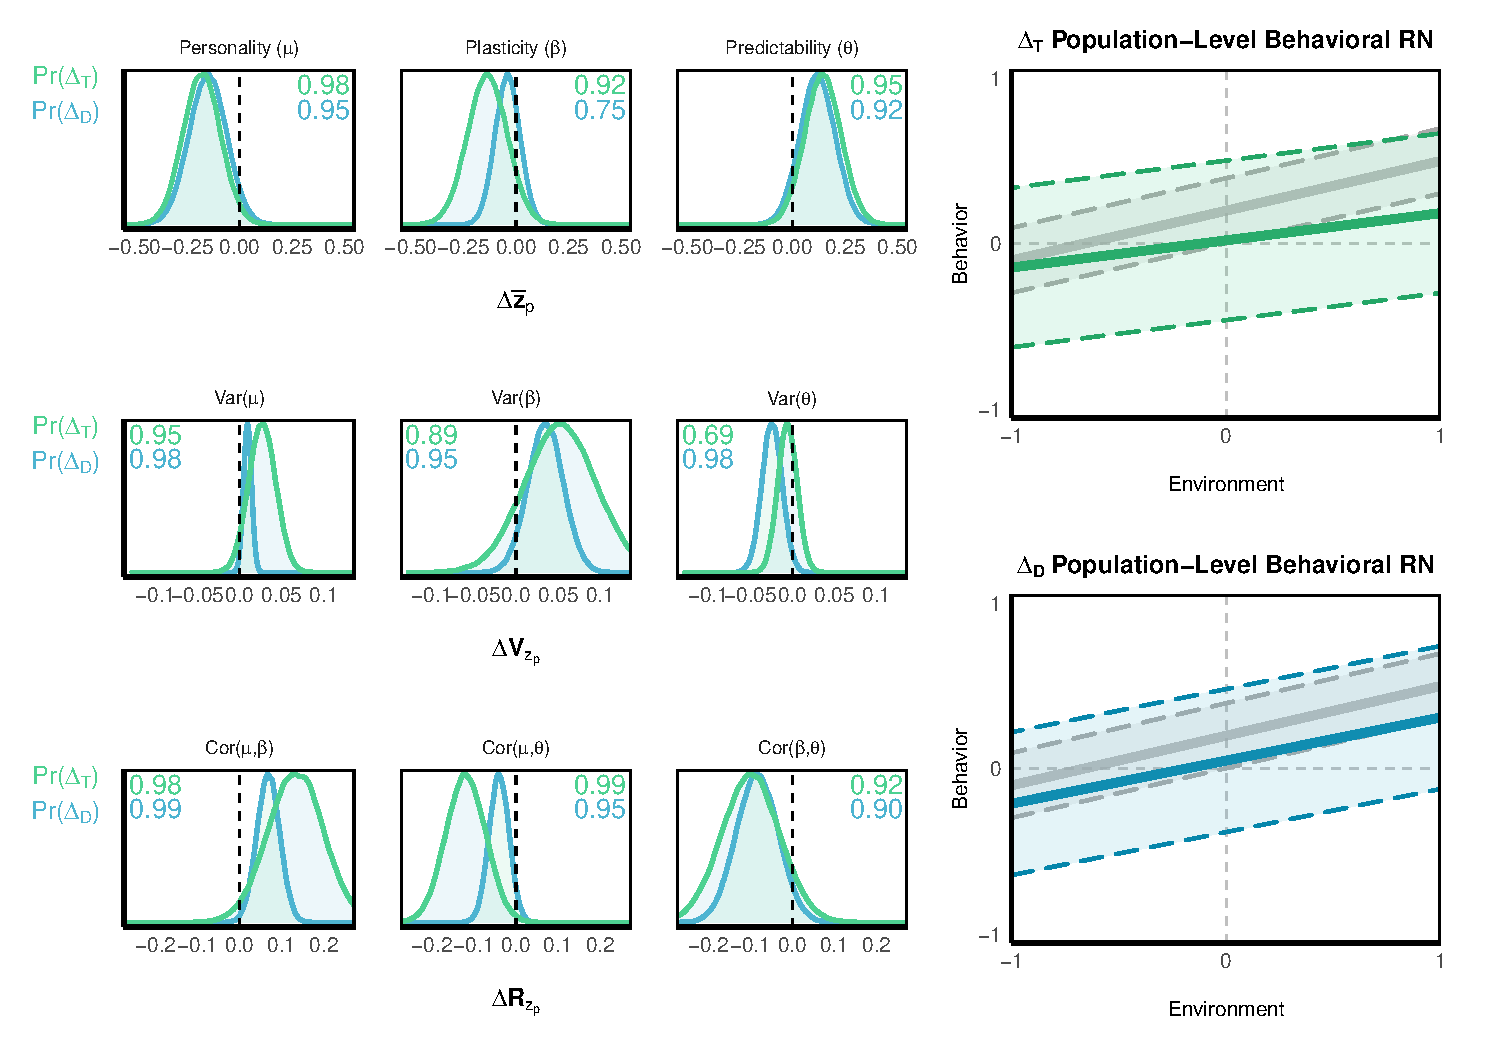
\includegraphics[scale=0.73]{fig3_2.pdf}
\caption{Proposed representation of multivariate selection on a behavioral RN. Plots are shown for the within-generation effects of a hypothetical selection event, where selection was characterized by a combination of directional, quadratic, and correlational fitness effects across RN parameters. Distinct outcomes are shown for the direct effects of selection ($\Delta_{\mathrm{D}}$) causing adaptation independent of trait covariation, as well as the total effects of selection ($\Delta_{\mathrm{T}}$) accounting for indirect effects due to phenotypic integration among RN parameters.  \\ \\ 
$\boldsymbol{Left \ panel}$: Three rows are shown for the distinct effects of multivariate selection on the average population RN parameter values ($\Delta \boldsymbol{\bar{z}}_\mathrm{p}$), individual variation in population RN values (represented by the population variance, $\Delta \boldsymbol{\mathrm{V}}_\mathrm{z_p}$), and the integration among RN parameters (represented by the population correlations, $\Delta \boldsymbol{\mathrm{R}}_\mathrm{z_p}$). Uncertainty around these predicted changes is captured by posterior distributions of each selection differential, with the posterior probability $\Pr(\Delta)$ supporting the expected direction of change for total and direct effects indicated in the top corner of each plot. If individual differences are adaptive, it is expected that selection will act to directly increase or maintain the population variance of RN parameters ($\Delta_{\mathrm{D}} \boldsymbol{\mathrm{V}}_\mathrm{z_p} \geq 0$); similarly, if trait integration is adaptive, selection will directly increase or maintain trait correlations (i.e. $\Delta_{\mathrm{D}} \boldsymbol{\mathrm{R}}_\mathrm{z_p} \geq 0$). Adaptation may nevertheless be constrained or accelerated by indirect effects due to phenotypic integration. In this hypothetical scenario, it can be seen that although selection is acting to decrease individual variation in predictability, $\mathrm{Pr}(\Delta_{\mathrm{D}}=0.98 )$, indirect effects lead to no clear expected change in the population variance, $\mathrm{Pr}(\Delta_{\mathrm{T}}=0.69 )$. Similarly, while there is only weak evidence of direct selection to decrease the mean plasticity in the population, $\mathrm{Pr}(\Delta_{\mathrm{D}}=0.75 )$, indirect effects are expected to cause a more pronounced change, $\mathrm{Pr}(\Delta_{\mathrm{D}}=0.92 )$.    \\ \\
$\boldsymbol{Right \ panel}$: The expected change in the shape of the population behavioral RN following selection. The population RN prior to selection is indicated by the grey line and band. Point estimates from the posterior distributions of $\Delta \boldsymbol{\bar{z}}_\mathrm{p}$ are used to visualize how direct and total selection effects shift the mean population RN across the relevant environmental gradient. The dashed, shaded bands indicate the $95\%$ credible intervals (i.e. $1.96*\uptheta$) capturing the expected levels of behavioral predictability in the population.
}
\label{fig:fig3}
\end{figure}

\hypertarget{simulation-based-calibration-of-proposed-models}{%
\section{Simulation-based calibration of proposed
models}\label{simulation-based-calibration-of-proposed-models}}

I used a simulation-based calibration (SBC) procedure to validate the
inferential performance of the proposed Bayesian models and assess
whether they provide unbiased estimators of selection. SBC is a
procedure for validating the performance of any Bayesian algorithm
across a broad range of possible parameter values, as defined by the
prior distributions of a generative model. This approach removes the
arbitrariness of setting a limited range of fixed parameter values for
assessing performance, which can lead to unexpected sources of bias
being overlooked in uninvestigated regions of parameter space (e.g.~rare
but possible combinations of RN correlations, standard deviations, and
selection coefficients). Instead, random parameter values are repeatedly
imputed during each MCMC iteration of model estimation for a large
number of simulations and visual inspection of the correspondence
between the generative distributions and subsequent posterior
distributions is used to detect any sources of bias, such as
overdispersion in the estimator or inconsistent performance for extreme
values. While a detailed explanation of SBC implementation and
interpretation is beyond the scope of the present study (see
\protect\hyperlink{ref-Talts2018}{Talts et al. 2018} for further
details), it suffices to say that a GLMM validated through SBC is an
unbiased Bayesian estimator. This method was, therefore, used to ensure
that empirical studies using the proposed models would be expected to
arrive at unbiased estimates over a plausible range of possible
parameter values.

Particular attention was given to the estimation of linear and nonlinear
selection coefficients during SBC, using 250 simulated datasets with 400
independent posterior samples each, resulting in the exploration of
100,000 possible random combinations of all model parameters. As
recommended by \protect\hyperlink{ref-Talts2018}{Talts et al.}
(\protect\hyperlink{ref-Talts2018}{2018}), visual inspection of the SBC
diagnostic plots demonstrated that the ranks of posterior selection
coefficients were consistent with a random, uniform distribution around
the prior simulated values, suggesting desirable performance indicative
of unbiased inference. Following the recommendation of
\protect\hyperlink{ref-Cook2006}{Cook, Gelman, and Rubin}
(\protect\hyperlink{ref-Cook2006}{2006}), I also further tested the
uniformity of the rank distribution by sorting ranks into eight evenly
distributed bins and applying a simple null-hypothesis test,
\(\chi^2(7)=6.06, P = 0.53\), further suggesting that coefficient ranks
were randomly and evenly distributed. In other words, posterior
inferences were not systematically upwardly or downwardly biased from
the true values, indicating that the proposed models are expected to
provide unbiased estimators of selection on behavioral RNs across a
broad range of parameter space.

\hypertarget{conclusion}{%
\section{Conclusion}\label{conclusion}}

Understanding the adaptive evolution of individual variation is an
exciting and bustling frontier in evolutionary ecology. Repeatable
individual differences in behavioral consistency, plasticity, and
predictability have now been demonstrated across a broad range of taxa
under a variety of ecological conditions. The challenge for behavioral
ecologists is thus no longer to simply document and describe
between-individual differences in behavior, but to instead test theory
explaining how and why these patterns are observed
(\protect\hyperlink{ref-Ding2020}{Dingemanse and Wright 2020}). It is
now well-established that a variety of non-adaptive mechanisms can
readily maintain repeatable phenotypic variability and trait
correlations within a population, particularly for traits with complex
genetic architectures. Therefore, the existence of such variation in
itself does not provide strong reason to suspect that natural selection
is acting to increase or maintain individuality within a population.
\protect\hyperlink{ref-Bierbach2017}{Bierbach, Laskowski, and Wolf}
(\protect\hyperlink{ref-Bierbach2017}{2017}), for example, found that
personality emerged in activity level among clonal fish raised in highly
controlled environmental conditions, likely as a result of developmental
noise. Similar findings have been obtained for clonal mice, where
individuality in behavior can result from subtle differences in
neurobiological and epigenetic responses toward standardized early
rearing environments (\protect\hyperlink{ref-Zocher2020}{Zocher et al.
2020}). Processes such as mutation-selection balance also remain
plausible explanations for the maintenance of non-adaptive behavioral
variation even in the presence of consistent stabilizing selection
(\protect\hyperlink{ref-Zhang2005}{Zhang and Hill 2005}), particularly
for complex traits with large mutational target sizes caused by highly
polygenic and pleiotropic developmental pathways
(\protect\hyperlink{ref-Houle1998}{Houle 1998};
\protect\hyperlink{ref-Boyle2017}{Boyle, Li, and Pritchard 2017}).
Empirical research in humans has, for example, provided support for the
role of mutation-selection balance in maintaining repeatable variation
in personality (\protect\hyperlink{ref-Verw2012}{Verweij et al. 2016}),
psychopathology (\protect\hyperlink{ref-Keller2008}{Keller 2008};
\protect\hyperlink{ref-Pard2018}{Pardiñas et al. 2018}), and general
intelligence (\protect\hyperlink{ref-Hill2018}{Hill et al. 2018}). In
light of these considerations, the mere existence of differential
personality, plasticity, and/or predictability within a population
should not be considered biologically surprising, nor should it be
considered particularly informative on its own for advancing behavioral
ecological theory (\protect\hyperlink{ref-Beekman2017}{Beekman and
Jordan 2017}). The onus thus remains on empiricists to demonstrate the
evolutionary relevance of individual variation within their study
system, as well as to identify the common mechanisms and selection
pressures that may facilitate or diminish its maintenance across
generations. While many such studies are now available (e.g.
\protect\hyperlink{ref-Ding2005}{Dingemanse and Réale 2005}; Le
\protect\hyperlink{ref-LC2015}{Cœur et al. 2015}; Le
\protect\hyperlink{ref-Gall2015}{Galliard, Paquet, and Mugabo 2015}),
there is a clear need for more phenotypic selection analyses on
behavioral RNs in the wild. As John Maynard
\protect\hyperlink{ref-Smith1978}{Smith}
(\protect\hyperlink{ref-Smith1978}{1978}) once noted, ``The most direct
way of testing a hypothesis about adaptation is to compare individuals
with different phenotypes, to see whether their fitnesses vary in the
way predicted by the hypothesis'' (p.~45).

A fundamental challenge for this research endeavor is to avoid
inferential bias caused by using BLUP point estimates of individuals'
latent personality, plasticity, and predictability parameters to predict
fitness (\protect\hyperlink{ref-Hadfield2010}{Hadfield et al. 2010}), as
these trait values are typically inferred with high degrees of
uncertainty from GLMMs. Previous attempts to address this issue
(\protect\hyperlink{ref-Hous2017}{Houslay and Wilson 2017}) have
proposed using random effects models to account for the uncertainty of
BLUPs, but this approach restricts analyses to the estimation of linear
correlations and covariances among RNs and fitness. Ignoring non-linear
associations fundamentally inhibits researchers' capacity to study
adaptive individual differences, as persistent directional/linear
selection is expected to diminish rather than promote individuality
within a population due to the exhaustion of fitness-relevant additive
genetic variance (\protect\hyperlink{ref-Walsh2009}{Walsh and Blows
2009}). To overcome this limitation, the present study developed and
investigated the properties of novel Bayesian models for studying
nonlinear selection on behavioral RNs. These models synthesize the
Lande-Arnold selection framework
(\protect\hyperlink{ref-Lande1983}{Lande and Arnold 1983}) with the GLMM
framework for quantifying individual variation
(\protect\hyperlink{ref-DingDocht2013}{Dingemanse and Dochtermann 2013})
into a single multi-response model, thus integrating uncertainty in
BLUPs and their effects into a comprehensive analysis. As a consequence,
various complex forms of nonlinear selection--such as stabilizing,
disruptive, balancing, and/or correlational selection--can be estimated
to test competing hypotheses of why variation in RNs persists within a
population. Given the challenge of visualizing high-dimensional
selection surfaces (\protect\hyperlink{ref-Phillips1989}{Phillips and
Arnold 1989}), I further proposed a simple method for visualizing the
expected direct and total effects of selection on the evolution of
behavioral RNs. This approach facilitates intuitive tests of adaptive
hypotheses on specific behavioral parameters, even in the presence of
high-dimensional phenotypes and complex selection surfaces.

It is important to note that selection differentials estimated from the
proposed models (Eq \ref{eq:1.2} \& Eq \ref{eq:2}) will be sensitive to
missing fitness-relevant phenotypes or functional relationships, which
is a deeper issue with any trait-based model of selection and
evolutionary change (\protect\hyperlink{ref-Morrissey2010}{Morrissey,
Kruuk, and Wilson 2010}). However, behavioral ecologists are generally
interested in developing and testing adaptive theory of selection,
rather than most accurately predicting patterns of microevolutionary
change within a population. By focusing on trait-based models, rather
than pure variance-partitioning analyses, broader comparative patterns
of adaptation and selection can be better recognized and evaluated (e.g.
\protect\hyperlink{ref-Kingsolver2001}{Kingsolver et al. 2001}).
Nevertheless, it is often useful to compare the predicted mean changes
in phenotypic values between trait- and variance-partitioning models,
which can be used to assess the magnitude of effects that are being
overlooked with the fixed effects analysis
(\protect\hyperlink{ref-Morrissey2012}{Morrissey et al. 2012}). The
random effect correlation models proposed by
\protect\hyperlink{ref-Hous2017}{Houslay and Wilson}
(\protect\hyperlink{ref-Hous2017}{2017}) can thus provide complimentary
analyses to the models presented here. As discussed above, exploratory,
non-parametric analyses can then be employed to detect and better
characterize any unspecified nonlinear functions on fitness, which can
subsequently be integrated into the parametric model. In this way, the
goals of prediction and explanation, while distinct and in many cases
best suited to different modelling approaches
(\protect\hyperlink{ref-Shmueli2010}{Shmueli 2010}), can nonetheless be
integrated to better inform our understanding of microevolutionary
change. The proposed modeling framework should, therefore, readily
enhance tests of adaptive theory in the wild.

\pagebreak

\hypertarget{references}{%
\section*{References}\label{references}}
\addcontentsline{toc}{section}{References}

\hypertarget{refs}{}
\begin{CSLReferences}{1}{0}
\leavevmode\hypertarget{ref-Adolf2007}{}%
Adolph, S. C., and J. S. Hardin. 2007. {``Estimating Phenotypic
Correlations: Correcting for Bias Due to Intraindividual Variability.''}
\emph{Functional Ecology} 21: 178--84.

\leavevmode\hypertarget{ref-Amrhein2019}{}%
Amrhein, V., D. Trafimow, and S. Greenland. 2019. {``Inferential
Statistics as Descriptive Statistics: There Is No Replication Crisis If
We Don't Expect Replication.''} \emph{The American Statistician} 73:
262--70.

\leavevmode\hypertarget{ref-Araya2014}{}%
Araya-Ajoy, Y. G., and N. J. Dingemanse. 2014. {``Characterizing
Behavioural {`Characters'}: An Evolutionary Framework.''}
\emph{Proceedings of the Royal Society B} 281: 20132645.

\leavevmode\hypertarget{ref-Araya2020}{}%
Araya-Ajoy, Y. G., D. F. Westneat, and J. Wright. 2020. {``Pathways to
Social Evolution and Their Evolutionary Feedbacks.''} \emph{Evolution}
74: 1894--1907.

\leavevmode\hypertarget{ref-Bates2014}{}%
Bates, D., M. Mächler, B. Bolker, and S. Walker. 2014. {``Fitting Linear
Mixed-Effects Models Using Lme4.''} \emph{arXiv Preprint} 1406.5823.

\leavevmode\hypertarget{ref-Beekman2017}{}%
Beekman, M., and L. A. Jordan. 2017. {``Does the Field of Animal
Personality Provide Any New Insights for Behavioral Ecology?''}
\emph{Behavioral Ecology} 28: 617--23.

\leavevmode\hypertarget{ref-Bell2009}{}%
Bell, A. M., S. J. Hankison, and K. L. Laskowski. 2009. {``The
Repeatability of Behaviour: A Meta-Analysis.''} \emph{Animal Behaviour}
77: 771--83.

\leavevmode\hypertarget{ref-Bierbach2017}{}%
Bierbach, D., K. L. Laskowski, and M. Wolf. 2017. {``Behavioural
Individuality in Clonal Fish Arises Despite Near-Identical Rearing
Conditions.''} \emph{Nature Communications} 8: 1--7.

\leavevmode\hypertarget{ref-Biro2013}{}%
Biro, P. A., and B. Adriaenssens. 2013. {``Predictability as a
Personality Trait: Consistent Differences in Intraindividual Behavioral
Variation.''} \emph{The American Naturalist} 182: 621--29.

\leavevmode\hypertarget{ref-Blows2003}{}%
Blows, M. W. 2003. {``Measuring Nonlinear Selection.''} \emph{The
American Naturalist} 2003: 815--20.

\leavevmode\hypertarget{ref-Blows2007}{}%
---------. 2007. {``A Tale of Two Matrices: Multivariate Approaches in
Evolutionary Biology.''} \emph{Journal of Evolutionary Biology} 20:
1--8.

\leavevmode\hypertarget{ref-Bollen2011}{}%
Bollen, K. A., and M. D. Noble. 2011. {``Structural Equation Models and
the Quantification of Behavior.''} \emph{Proceedings of the National
Academy of Sciences} 108: 15639--46.

\leavevmode\hypertarget{ref-Boyle2017}{}%
Boyle, E. A., Y. I. Li, and J. K. Pritchard. 2017. {``An Expanded View
of Complex Traits: From Polygenic to Omnigenic.''} \emph{Cell} 169:
1177--86.

\leavevmode\hypertarget{ref-Brehm2019}{}%
Brehm, A. M., A. Mortelliti, G. A. Maynard, and J. Zydlewski. 2019.
{``Land‐use Change and the Ecological Consequences of Personality in
Small Mammal.''} \emph{Ecology Letters} 22: 1387--95.

\leavevmode\hypertarget{ref-Briley2019}{}%
Briley, D. A., J. Livengood, J. Derringer, E. M. Tucker-Drob, R. C.
Fraley, and B. W. Roberts. 2019. {``Interpreting Behavior Genetic
Models: Seven Developmental Processes to Understand.''} \emph{Behavioral
Genetics} 49: 196--210.

\leavevmode\hypertarget{ref-Brodie2007}{}%
Brodie, E. D. III, and J. W. McGlothlin. 2007. {``A Cautionary Tale of
Two Matrices: The Duality of Multivariate Abstraction.''} \emph{Journal
of Evolutionary Biology} 20: 9--14.

\leavevmode\hypertarget{ref-Brommer2013}{}%
Brommer, J. E. 2013. {``On Between-Individual and Residual (Co)
Variances in the Study of Animal Personality: Are You Willing to Take
the 'Individual Gambit'?''} \emph{Behavioral Ecology and Sociobiology}
67: 1027--32.

\leavevmode\hypertarget{ref-brms2017}{}%
Bürkner, P. C. 2017. {``Advanced Bayesian Multilevel Modeling with the r
Package Brms.''} \emph{arXiv} 1705.11123.

\leavevmode\hypertarget{ref-Stan}{}%
Carpenter, B., A. Gelman, M. D. Hoffman, D. Lee, B. Goodrich, M.
Betancourt, and... A. Riddell. 2017. {``Stan: A Probabilistic
Programming Language.''} \emph{Journal of Statistical Software} 74.
\url{https://www.jstatsoft.org/article/view/v076i01}.

\leavevmode\hypertarget{ref-Cauch2018}{}%
Cauchoix, M., P. K. Y. Chow, J. O. Van Horik, C. M. Atance, E. J.
Barbeau,...G. Barragan-Jason, and L. Cauchard. 2018. {``The
Repeatability of Cognitive Performance: A Meta-Analysis.''}
\emph{Philosophical Transactions of the Royal Society B} 373: 20170281.

\leavevmode\hypertarget{ref-Conner2007}{}%
Conner, J. K. 2007. {``A Tale of Two Methods: Putting Biology Before
Statistics in the Study of Phenotypic Evolution.''} \emph{Journal of
Evolutionary Biology} 20: 17--19.

\leavevmode\hypertarget{ref-Conner2012}{}%
---------. 2012. {``Quantitative Genetic Approaches to Evolutionary
Constraint: How Useful?''} \emph{Evolution} 66: 3313--20.

\leavevmode\hypertarget{ref-Cook2006}{}%
Cook, S. R., A. Gelman, and D. B. Rubin. 2006. {``Validation of Software
for Bayesian Models Using Posterior Quantiles.''} \emph{Journal of
Computational and Graphical Statistics} 15: 675--92.

\leavevmode\hypertarget{ref-LC2015}{}%
Cœur, C. C., M. Thibault, B. Pisanu, S. Thibault, J. L. Chapuis, and E.
Baudry. 2015. {``Temporally Fluctuating Selection on a Personality Trait
in a Wild Rodent Population.''} \emph{Behavioral Ecology} 26: 1285--91.

\leavevmode\hypertarget{ref-Dall2014}{}%
Dall, S. R. X., and S. C. Griffith. 2014. {``An Empiricist Guide to
Animal Personality Variation in Ecology and Evolution.''}
\emph{Frontiers in Ecology and Evolution} 14: 3.

\leavevmode\hypertarget{ref-Darwin}{}%
Darwin, C. 1859. \emph{On the Origin of Species by Means of Natural
Selection}. London, UK: J. Murray.

\leavevmode\hypertarget{ref-Ding2021}{}%
Dingemanse, N. J., Y. G. Araya‐Ajoy, and D. F. Westneat. 2021. {``Most
Published Selection Gradients Are Underestimated: Why This Is and How to
Fix It.''} \emph{Evolution} Early View.

\leavevmode\hypertarget{ref-DingDocht2013}{}%
Dingemanse, N. J., and N. A. Dochtermann. 2013. {``Quantifying
Individual Variation in Behaviour: Mixed‐effect Modelling Approaches.''}
\emph{Journal of Animal Ecology} 82: 39--54.

\leavevmode\hypertarget{ref-Ding2010}{}%
Dingemanse, N. J., A. J. Kazem, D. Réale, and J. Wright. 2010.
{``Behavioural Reaction Norms: Animal Personality Meets Individual
Plasticity.''} \emph{Trends in Ecology and Evolution} 25: 81--89.

\leavevmode\hypertarget{ref-Ding2020b}{}%
Dingemanse, N. J., M. Moiron, Y. G. Araya‐Ajoy, A. Mouchet, and R. N.
Abbey‐Lee. 2020. {``Individual Variation in Age‐dependent Reproduction:
Fast Explorers Live Fast but Senesce Young?''} \emph{Journal of Animal
Ecology} 89: 601--13.

\leavevmode\hypertarget{ref-Ding2005}{}%
Dingemanse, N. J., and D. Réale. 2005. {``Natural Selection and Animal
Personality.''} \emph{Behaviour} 142: 1159--84.

\leavevmode\hypertarget{ref-Ding2020}{}%
Dingemanse, N. J., and J. Wright. 2020. {``Criteria for Acceptable
Studies of Animal Personality and Behavioural Syndromes.''}
\emph{Ethology} 126: 865--69.

\leavevmode\hypertarget{ref-Eis2011}{}%
Eisenegger, C., J. Haushofer, and E. Fehr. 2011. {``The Role of
Testosterone in Social Interaction.''} \emph{Trends in Cognitive
Sciences} 15: 263--71.

\leavevmode\hypertarget{ref-Ellison2004}{}%
Ellison, A. M. 2004. {``Bayesian Inference in Ecology.''} \emph{Ecology
Letters} 7: 509--20.

\leavevmode\hypertarget{ref-Fanson2019}{}%
Fanson, K. V., and P. A. Biro. 2015. {``Meta-Analytic Insights into
Factors Influencing the Repeatability of Hormone Levels in Agricultural,
Ecological, and Medical Fields.''} \emph{American Journal of
Physiology-Regulatory, Integrative and Comparative Physiology} 316:
R101--9.

\leavevmode\hypertarget{ref-Gall2015}{}%
Galliard, J. F. L., M. Paquet, and M. Mugabo. 2015. {``An Experimental
Test of Density-Dependent Selection on Temperament Traits of Activity,
Boldness and Sociability.''} \emph{Journal of Evolutionary Biology} 28:
1144--55.

\leavevmode\hypertarget{ref-Gelman2017}{}%
Gelman, A., and J. Carlin. 2017. {``Some Natural Solutions to the
p-Value Communication Problem---and Why They Won't Work.''}
\emph{Journal of the American Statistician} 112: 899--901.

\leavevmode\hypertarget{ref-Gelman2000}{}%
Gelman, A., and F. Tuerlinckx. 2000. {``Type s Error Rates for Classical
and Bayesian Single and Multiple Comparison Procedures.''}
\emph{Computational Statistics} 15: 373--90.

\leavevmode\hypertarget{ref-Gelman2020}{}%
Gelman, A., A. Vehtari, D. Simpson, C. C. Margossian, B. Carpenter, Y.
Yao, and... M. Modrák. 2020. {``Bayesian Workflow.''} \emph{arXiv
Preprint} arXiv:2011.01808. \url{https://arxiv.org/abs/2011.01808}.

\leavevmode\hypertarget{ref-Gomulk2018}{}%
Gomulkiewicz, R., J. G. Kingsolver, P. A. Carter, and N. Heckman. 2018.
{``Variation and Evolution of Function-Valued Traits.''} \emph{Annual
Review of Ecology, Evolution, and Systematics} 49: 139--64.

\leavevmode\hypertarget{ref-Green2016}{}%
Greenland, S., S. J. Senn, K. J. Rothman, J. B. Carlin, C. Poole, S. N.
Goodman, and D. G. Altman. 2016. {``Statistical Tests, p Values,
Confidence Intervals, and Power: A Guide to Misinterpretations.''}
\emph{European Journal of Epidemiology} 31: 337--50.

\leavevmode\hypertarget{ref-Gurven2014}{}%
Gurven, M., C. von Rueden, J. Stieglitz, H. Kaplan, and D. E. Rodriguez.
2014. {``The Evolutionary Fitness of Personality Traits in a Small-Scale
Subsistence Society.''} \emph{Evolution and Human Behavior} 35: 17--25.

\leavevmode\hypertarget{ref-Hadfield2017}{}%
Hadfield, J. D., and C. E. Thomson. 2017. {``Interpreting Selection When
Individuals Interact.''} \emph{Methods in Ecology and Evolution} 8:
688--99.

\leavevmode\hypertarget{ref-Hadfield2010}{}%
Hadfield, J. D., A. J. Wilson, D. Garant, and B. C. Sheldon. 2010.
{``The Misuse of BLUP in Ecology and Evolution.''} \emph{The American
Naturalist} 175: 116--25.

\leavevmode\hypertarget{ref-Hill2018}{}%
Hill, W. D., R. C. Arslan, C. Xia, M. Luciano, C. Amador,...P. Navarro,
and L. Penke. 2018. {``Genomic Analysis of Family Data Reveals
Additional Genetic Effects on Intelligence and Personality.''}
\emph{Molecular Psychiatry} 23: 2347--62.

\leavevmode\hypertarget{ref-Houle1998}{}%
Houle, D. 1998. {``How Should We Explain Variation in the Genetic
Variance of Traits?''} \emph{Genetica} 102: 241--53.

\leavevmode\hypertarget{ref-Hous2017}{}%
Houslay, T. M., and A. J. Wilson. 2017. {``Avoiding the Misuse of BLUP
in Behavioural Ecology.''} \emph{Behavioral Ecology} 28: 948--52.

\leavevmode\hypertarget{ref-Jaeggi2016}{}%
Jaeggi, A. V., K. J. Boose, F. J. White, and M. Gurven. 2016.
{``Obstacles and Catalysts of Cooperation in Humans, Bonobos, and
Chimpanzees: Behavioural Reaction Norms Can Help Explain Variation in
Sex Roles, Inequality, War and Peace.''} \emph{Behaviour} 153: 1015--52.

\leavevmode\hypertarget{ref-Keller2008}{}%
Keller, M. C. 2008. {``The Evolutionary Persistence of Genes That
Increase Mental Disorders Risk.''} \emph{Current Directions in
Psychological Science} 17: 395--99.

\leavevmode\hypertarget{ref-Kingsolver2001}{}%
Kingsolver, J. G., H. E. Hoekstra, J. M. Hoekstra, D. Berrigan, S. N.
Vignieri,...C. E. Hill, and P. Beerli. 2001. {``The Strength of
Phenotypic Selection in Natural Populations.''} \emph{The American
Naturalist} 157: 245--51.

\leavevmode\hypertarget{ref-Lande1983}{}%
Lande, R., and S. J. Arnold. 1983. {``The Measurement of Selection on
Correlated Characters.''} \emph{Evolution} 37: 1210--26.

\leavevmode\hypertarget{ref-Lemoine2019}{}%
Lemoine, N. P. 2019. {``Moving Beyond Noninformative Priors: Why and How
to Choose Weakly Informative Priors in Bayesian Analyses.''}
\emph{Oikos} 128.
\url{https://onlinelibrary.wiley.com/doi/full/10.1111/oik.05985}.

\leavevmode\hypertarget{ref-Martin2021}{}%
Martin, J. S., and A. V. Jaeggi. 2021. {``Social Animal Models for
Quantifying Plasticity, Assortment, and Selection on Interacting
Phenotypes.''} \emph{In Review}.

\leavevmode\hypertarget{ref-Martin2019}{}%
Martin, J. S., J. J. Massen, V. Šlipogor, T. Bugnyar, A. V. Jaeggi, and
S. E. Koski. 2019. {``The EGA+ GNM Framework: An Integrative Approach to
Modelling Behavioural Syndromes.''} \emph{Methods in Ecology and
Evolution} 10: 245--57.

\leavevmode\hypertarget{ref-Mathuru2012}{}%
Mathuru, A. S., C. Kibat, W. F. Cheong, G. Shui, M. R. Wenk, R. W.
Friedrich, and S. Jesuthasan. 2012. {``Chondroitin Fragments Are
Odorants That Trigger Fear Behavior in Ffsh.''} \emph{Current Biology}
22: 538--54.

\leavevmode\hypertarget{ref-Rethinking}{}%
McElreath, R. 2020. \emph{Statistical Rethinking: A Bayesian Course with
Examples in r and Stan}. 2nd ed. CRC Press.
\url{https://xcelab.net/rm/statistical-rethinking/}.

\leavevmode\hypertarget{ref-McNamara2020}{}%
McNamara, J. M., and O. Leimar. 2020. \emph{Game Theory in Biology}.
Oxford, UK: Oxford University Press.

\leavevmode\hypertarget{ref-McShane2019}{}%
McShane, B. B., D. Gal, A. Gelman, C. Robert, and J. L. Tackett. 2019.
{``Abandon Statistical Significance.''} \emph{The American Naturalist}
73: 235--45.

\leavevmode\hypertarget{ref-Meehl1978}{}%
Meehl, P. E. 1978. {``Theoretical Risks and Tabular Asterisks: Sir Karl,
Sir Ronald, and the Slow Progress of Soft Psychology.''} \emph{Journal
of Consulting and Clinical Psychology} 46: 806--34.

\leavevmode\hypertarget{ref-Morrissey2014}{}%
Morrissey, M. B. 2014. {``In Search of the Best Methods for Multivariate
Selection Analysis.''} \emph{Methods in Ecology and Evolution} 5:
1095--1109.

\leavevmode\hypertarget{ref-Morrissey2010}{}%
Morrissey, M. B., L. E. B. Kruuk, and A. J. Wilson. 2010. {``The Danger
of Applying the Breeder's Equation in Observational Studies of Natural
Populations.''} \emph{Journal of Evolutionary Biology} 23: 2277--88.

\leavevmode\hypertarget{ref-Morrissey2012}{}%
Morrissey, M. B., D. J. Parker, P. Korsten, J. M. Pemberton, L. E. B.
Kruuk, and A. J. Wilson. 2012. {``The Prediction of Adaptive Evolution:
Empirical Application of the Secondary Theorem of Selection and
Comparison to the Breeder's Equation.''} \emph{Evolution} 66:
2399--2410.

\leavevmode\hypertarget{ref-Morrissey2013}{}%
Morrissey, M. B., and K. Sakrejda. 2013. {``Unification of
Regression-Based Methods for the Analysis of Natural Selection.''}
\emph{Evolution} 67: 2094--2100.

\leavevmode\hypertarget{ref-Naka2010}{}%
Nakagawa, S., and H. Schielzeth. 2010. {``Repeatability for Gaussian and
Non‐gaussian Data: A Practical Guide for Biologists.''} \emph{Biological
Reviews} 85: 935--56.

\leavevmode\hypertarget{ref-Nelder1972}{}%
Nelder, J. A., and R. W. Wedderburn. 1972. {``Generalized Linear
Models.''} \emph{Journal of the Royal Statistical Society: Series A}
135: 370--84.

\leavevmode\hypertarget{ref-Nettle2010}{}%
Nettle, D., and L. Penke. 2010. {``Personality: Bridging the Literatures
from Human Psychology and Behavioural Ecology.''} \emph{Philosophical
Transactions of the Royal Society B} 365: 4043--50.

\leavevmode\hypertarget{ref-Niem2018}{}%
Niemelä, P. T., and N. J. Dingemase. 2018. {``Meta-Analysis Reveals Weak
Associations Between Intrinsic State and Personality.''}
\emph{Proceedings of the Royal Society B} 285: 20172823.

\leavevmode\hypertarget{ref-Nus2007}{}%
Nussey, D. H., A. J. Wilson, and J. E. Brommer. 2007. {``The
Evolutionary Ecology of Individual Phenotypic Plasticity in Wild
Populations.''} \emph{Journal of Evolutionary Biology} 20: 831--44.

\leavevmode\hypertarget{ref-Okasha2020}{}%
Okasha, S., and J. Otsuka. 2020. {``The Price Equation and the Causal
Analysis of Evolutionary Change.''} \emph{Philosophical Transactions of
the Royal Society B} 375: 20190365.

\leavevmode\hypertarget{ref-Pard2018}{}%
Pardiñas, A. F., P. Holmans, A. J. Pocklington, V. Escott-Price, S.
Ripke,...N. Carrera, and J. T. Walters. 2018. {``Common Schizophrenia
Alleles Are Enriched in Mutation-Intolerant Genes and in Regions Under
Strong Background Selection.''} \emph{Nature Genetics} 50: 381--89.

\leavevmode\hypertarget{ref-Pedersen2019}{}%
Pedersen, E. J., D. L. Miller, G. L. Simpson, and N. Ross. 2019.
{``Hierarchical Generalized Additive Models in Ecology: An Introduction
with Mgcv.''} \emph{PeerJ} 7: e6876.

\leavevmode\hypertarget{ref-Phillips1989}{}%
Phillips, P. C., and S. J. Arnold. 1989. {``Visualizing Multivariate
Selection.''} \emph{Evolution} 43: 1209--22.

\leavevmode\hypertarget{ref-Piir2017}{}%
Piironen, J., and A. Vehtari. 2017. {``Sparsity Information and
Regularization in the Horseshoe and Other Shrinkage Priors.''}
\emph{Electronic Journal of Statistics} 22: 5018--51.

\leavevmode\hypertarget{ref-Pol2009}{}%
Pol, M. van de, and J. Wright. 2009. {``A Simple Method for
Distinguishing Within- Versus Between-Subject Effects Using Mixed
Models.''} \emph{Animal Behaviour} 77: 753--58.

\leavevmode\hypertarget{ref-Postma2006}{}%
Postma, E. 2006. {``Implications of the Difference Between True and
Predicted Breeding Values for the Study of Natural Selection and
Micro‐evolution.''} \emph{Journal of Evolutionary Biology} 19: 309--20.

\leavevmode\hypertarget{ref-Queller2011}{}%
Queller, D. C. 2011. {``Expanded Social Fitness and Hamilton's Rule for
Kin, Kith, and Kind.''} \emph{Proceedings of the National Academy of
Sciences USA} 108: 10792--99.

\leavevmode\hypertarget{ref-Rbase}{}%
R Core Team. 2020. \emph{R: A Language and Environment for Statistical
Computing}. Vienna, Austria: R Foundation for Statistical Computing.
\url{https://www.R-project.org}.

\leavevmode\hypertarget{ref-Roy2018}{}%
Royauté, R., M. A. Berdal, C. R. Garrison, and N. A. Dochtermann. 2018.
{``A Meta-Analysis of the Pace-of-Life Syndrome Hypothesis.''}
\emph{Behavioral Ecology and Sociobiology} 72: 1--10.

\leavevmode\hypertarget{ref-Roy2020}{}%
Royauté, R., A. Hedrick, and N. A. Dochtermann. 2020. {``Behavioural
Syndromes Shape Evolutionary Trajectories via Conserved Genetic
Architecture.''} \emph{Proceedings of the Royal Society B} 287:
20200183.

\leavevmode\hypertarget{ref-Rueden2015}{}%
Rueden, C. R., A. W. Lukaszewski, and M. Gurven. 2015. {``Adaptive
Personality Calibration in a Human Society: Effects of Embodied Capital
on Prosocial Traits.''} \emph{Behavioral Ecology} 26: 1071--82.

\leavevmode\hypertarget{ref-Scherer2018}{}%
Scherer, U., M. Kuhnhardt, and W. Schuett. 2018. {``Predictability Is
Attractive: Female Preference for Behaviourally Consistent Males but No
Preference for the Level of Male Aggression in a Bi-Parental Cichlid.''}
\emph{PloS One} 13: e0195766.

\leavevmode\hypertarget{ref-Schiel2020}{}%
Schielzeth, H., N. J. Dingemanse, S. Nakagawa, D. F. Westneat, H.
Allegue, C. Teplitsky, and Y. G. Araya-Ajoy. 2020. {``Robustness of
Linear Mixed Effects Models to Violations of Distributional
Assumptions.''} \emph{Methods in Ecology and Evolution} 11: 1141--52.

\leavevmode\hypertarget{ref-Schluter1994}{}%
Schluter, D., and D. Nychka. 1994. {``Exploring Fitness Surfaces.''}
\emph{The American Naturalist} 143: 597--616.

\leavevmode\hypertarget{ref-Shmueli2010}{}%
Shmueli, G. 2010. {``To Explain or to Predict?''} \emph{Statistical
Science} 25: 289--310.

\leavevmode\hypertarget{ref-Sih2015}{}%
Sih, A., K. J. Mathot, M. Moirón, P. O. Montiglio, M. Wolf, and N. J.
Dingemanse. 2015. {``Animal Personality and State--Behaviour Feedbacks:
A Review and Guide for Empiricists.''} \emph{Trends in Ecology and
Evolution} 30: 50--60.

\leavevmode\hypertarget{ref-Smith1978}{}%
Smith, J. M. 1978. {``Optimization Theory in Evolution.''} \emph{Annual
Review of Ecology and Systematics} 9: 31--56.

\leavevmode\hypertarget{ref-Spearman1904}{}%
Spearman, C. 1904. {``The Proof and Measurement of Association Between
Two Things.''} \emph{The American Journal of Psychology} 15: 72--101.

\leavevmode\hypertarget{ref-Stamps2016}{}%
Stamps, J. A. 2016. {``Individual Differences in Behavioural
Plasticities.''} \emph{Biological Reviews} 91: 534--67.

\leavevmode\hypertarget{ref-Stinch2008}{}%
Stinchcombe, J. R., A. F. Agrawal, P. A. Hohenlohe, S. J. Arnold, and M.
W. Blows. 2008. {``Estimating Nonlinear Selection Gradients Using
Quadratic Regression Coefficients: Double or Nothing?''}
\emph{Evolution} 68.
\url{https://onlinelibrary.wiley.com/doi/full/10.1111/evo.12321}.

\leavevmode\hypertarget{ref-Stinch2014}{}%
Stinchcombe, J. R., A. K. Simonsen, and M. W. Blows. 2014. {``Estimating
Uncertainty in Multivariate Responses to Selection.''} \emph{Evolution}
68. \url{https://onlinelibrary.wiley.com/doi/full/10.1111/evo.12321}.

\leavevmode\hypertarget{ref-Talts2018}{}%
Talts, S., M. Betancourt, D. Simpson, A. Vehtari, and A. Gelman. 2018.
{``Validating Bayesian Inference Algorithms with Simulation-Based
Calibration.''} \emph{arXiv Preprint} 1804.06788.

\leavevmode\hypertarget{ref-Tooby1990}{}%
Tooby, J., and L. Cosmides. 1990. {``On the Universality of Human Nature
and the Uniqueness of the Individual: The Role of Genetics and
Adaptation.''} \emph{Journal of Personality} 58: 17--67.

\leavevmode\hypertarget{ref-Verw2012}{}%
Verweij, K. J., J. Yang, J. Lahti, J. Veijola, M. Hintsanen,...L.
Pulkki‐Råback, and B. P. Zietsch. 2016. {``General Methods for
Evolutionary Quantitative Genetic Inference from Generalized Mixed
Models.''} \emph{Genetics} 204: 1281--94.

\leavevmode\hypertarget{ref-Vill2016}{}%
Villemereuil, P. de, H. Schielzeth, S. Nakagawa, and M. Morrissey. 2016.
{``General Methods for Evolutionary Quantitative Genetic Inference from
Generalized Mixed Models.''} \emph{Genetics} 204: 1281--94.

\leavevmode\hypertarget{ref-Walsh2009}{}%
Walsh, B., and M. Blows. 2009. {``Abundant Genetic Variation + Strong
Selection = Multivariate Genetic Constraints: A Geometric View of
Adaptation.''} \emph{Annual Review of Ecology, Evolution, and
Systematics} 40: 41--59.

\leavevmode\hypertarget{ref-Westneat2015}{}%
Westneat, D. F., J. Wright, and N. J. Dingemanse. 2015. {``The Biology
Hidden Inside Residual Within‐individual Phenotypic Variation.''}
\emph{Biological Reviews} 90: 729--43.

\leavevmode\hypertarget{ref-Wolf2010}{}%
Wolf, M., and F. J. Weissing. 2010. {``An Explanatory Framework for
Adaptive Personality Differences.''} \emph{Philosophical Transactions of
the Royal Society B} 365: 3959--68.

\leavevmode\hypertarget{ref-Wolf2012}{}%
---------. 2012. {``Animal Personalities: Consequences for Ecology and
Evolution.''} \emph{Trends in Ecology \& Evolution} 27: 452--61.

\leavevmode\hypertarget{ref-Wright2019}{}%
Wright, J., G. H. Bolstad, Y. G. Araya‐Ajoy, and N. J. Dingemanse. 2019.
{``Life‐history Evolution Under Fluctuating Density‐dependent Selection
and the Adaptive Alignment of Pace‐of‐life Syndromes.''}
\emph{Biological Reviews} 94: 230--47.

\leavevmode\hypertarget{ref-Zhang2005}{}%
Zhang, X. S., and W. G. Hill. 2005. {``Genetic Variability Under
Mutation Selection Balance.''} \emph{Trends in Ecology \& Evolution} 20:
468--70.

\leavevmode\hypertarget{ref-Zocher2020}{}%
Zocher, S., S. Schilling, A. N. Grzyb, V. S. Adusumilli, J. B. Lopes,...
S. Günther, and G. Kempermann. 2020. {``Early-Life Environmental
Enrichment Generates Persistent Individualized Behavior in Mice.''}
\emph{Science Advances} 6: eabb1478.

\end{CSLReferences}

\bibliographystyle{unsrt}
\bibliography{mybibfile.bib}


\end{document}
